\documentclass{scrartcl}
\usepackage{textcomp}
\usepackage{graphicx}
\usepackage{caption}
\usepackage{subcaption}
\usepackage[skip=2pt,font=scriptsize]{caption}
\usepackage[authoryear]{natbib}
\usepackage{gensymb}
\usepackage{amssymb,amsmath}
\usepackage{wrapfig}
\usepackage[toc,page]{appendix}
\usepackage{verbatim}
\usepackage{import}
\usepackage{rotating}
\usepackage{amsmath}
\usepackage{float}
\usepackage{lineno}
\linenumbers*[1]
\usepackage[top=0.5in, bottom=1.25in, left=1.25in, right=1.25in]{geometry}
%\usepackage[caption=false]{subfig}
\title{The Mantle Wedge: Dynamic Controls on Chemistry\\ 9 month report}
\author{Alexander Perrin}
\begin{document}
\section{Sample selection}
\begin{itemize}
\item Seven scoria samples.
\item Correct for post entrapment crystallisation, in the same way as . This correction assumes a constant K $_{D}$
\item Looked for trends Al$_2$O$_3$ vs MgO/Cao to identify samples that had only undergone olivine fractionation.
\item Added back in olivine in 0.1\% increments until in equilibrium with Mg\#=0.9 mantle. Required on average 22\% olivine. Excluded samples that required greater than 30\% addition. Assume Fe$^3+$/Fe$_total$=0.25.
\item Total of 20 samples from their samples, and 15 from \cite{shaw2008hydrogen}.
\item Melt inclusions thought to represent more primitive magma compositions \cite{schiano2003primitive} - \cite{kelley2010mantle} samples are on average $\sim$1 GPa deeper - can this tell us about magma evolution?
\end{itemize}

\section{Melt fraction calculations}
\begin{itemize}
\item Based on TiO$_2$/Y ratios, choose a source TiO$_2$ concentration of 0.123wt\%, slightly more depleted than DMM.
\item As do not know pre-eruptive H\textsubscript{2}O in our samples, there is uncertainty in melt fractions. See figure 
\end{itemize}



%/data/ap4909/30.10.2013-hot_cold_geochem/sample_testing/southern_marianas/kelley/mf_vs_ti.py
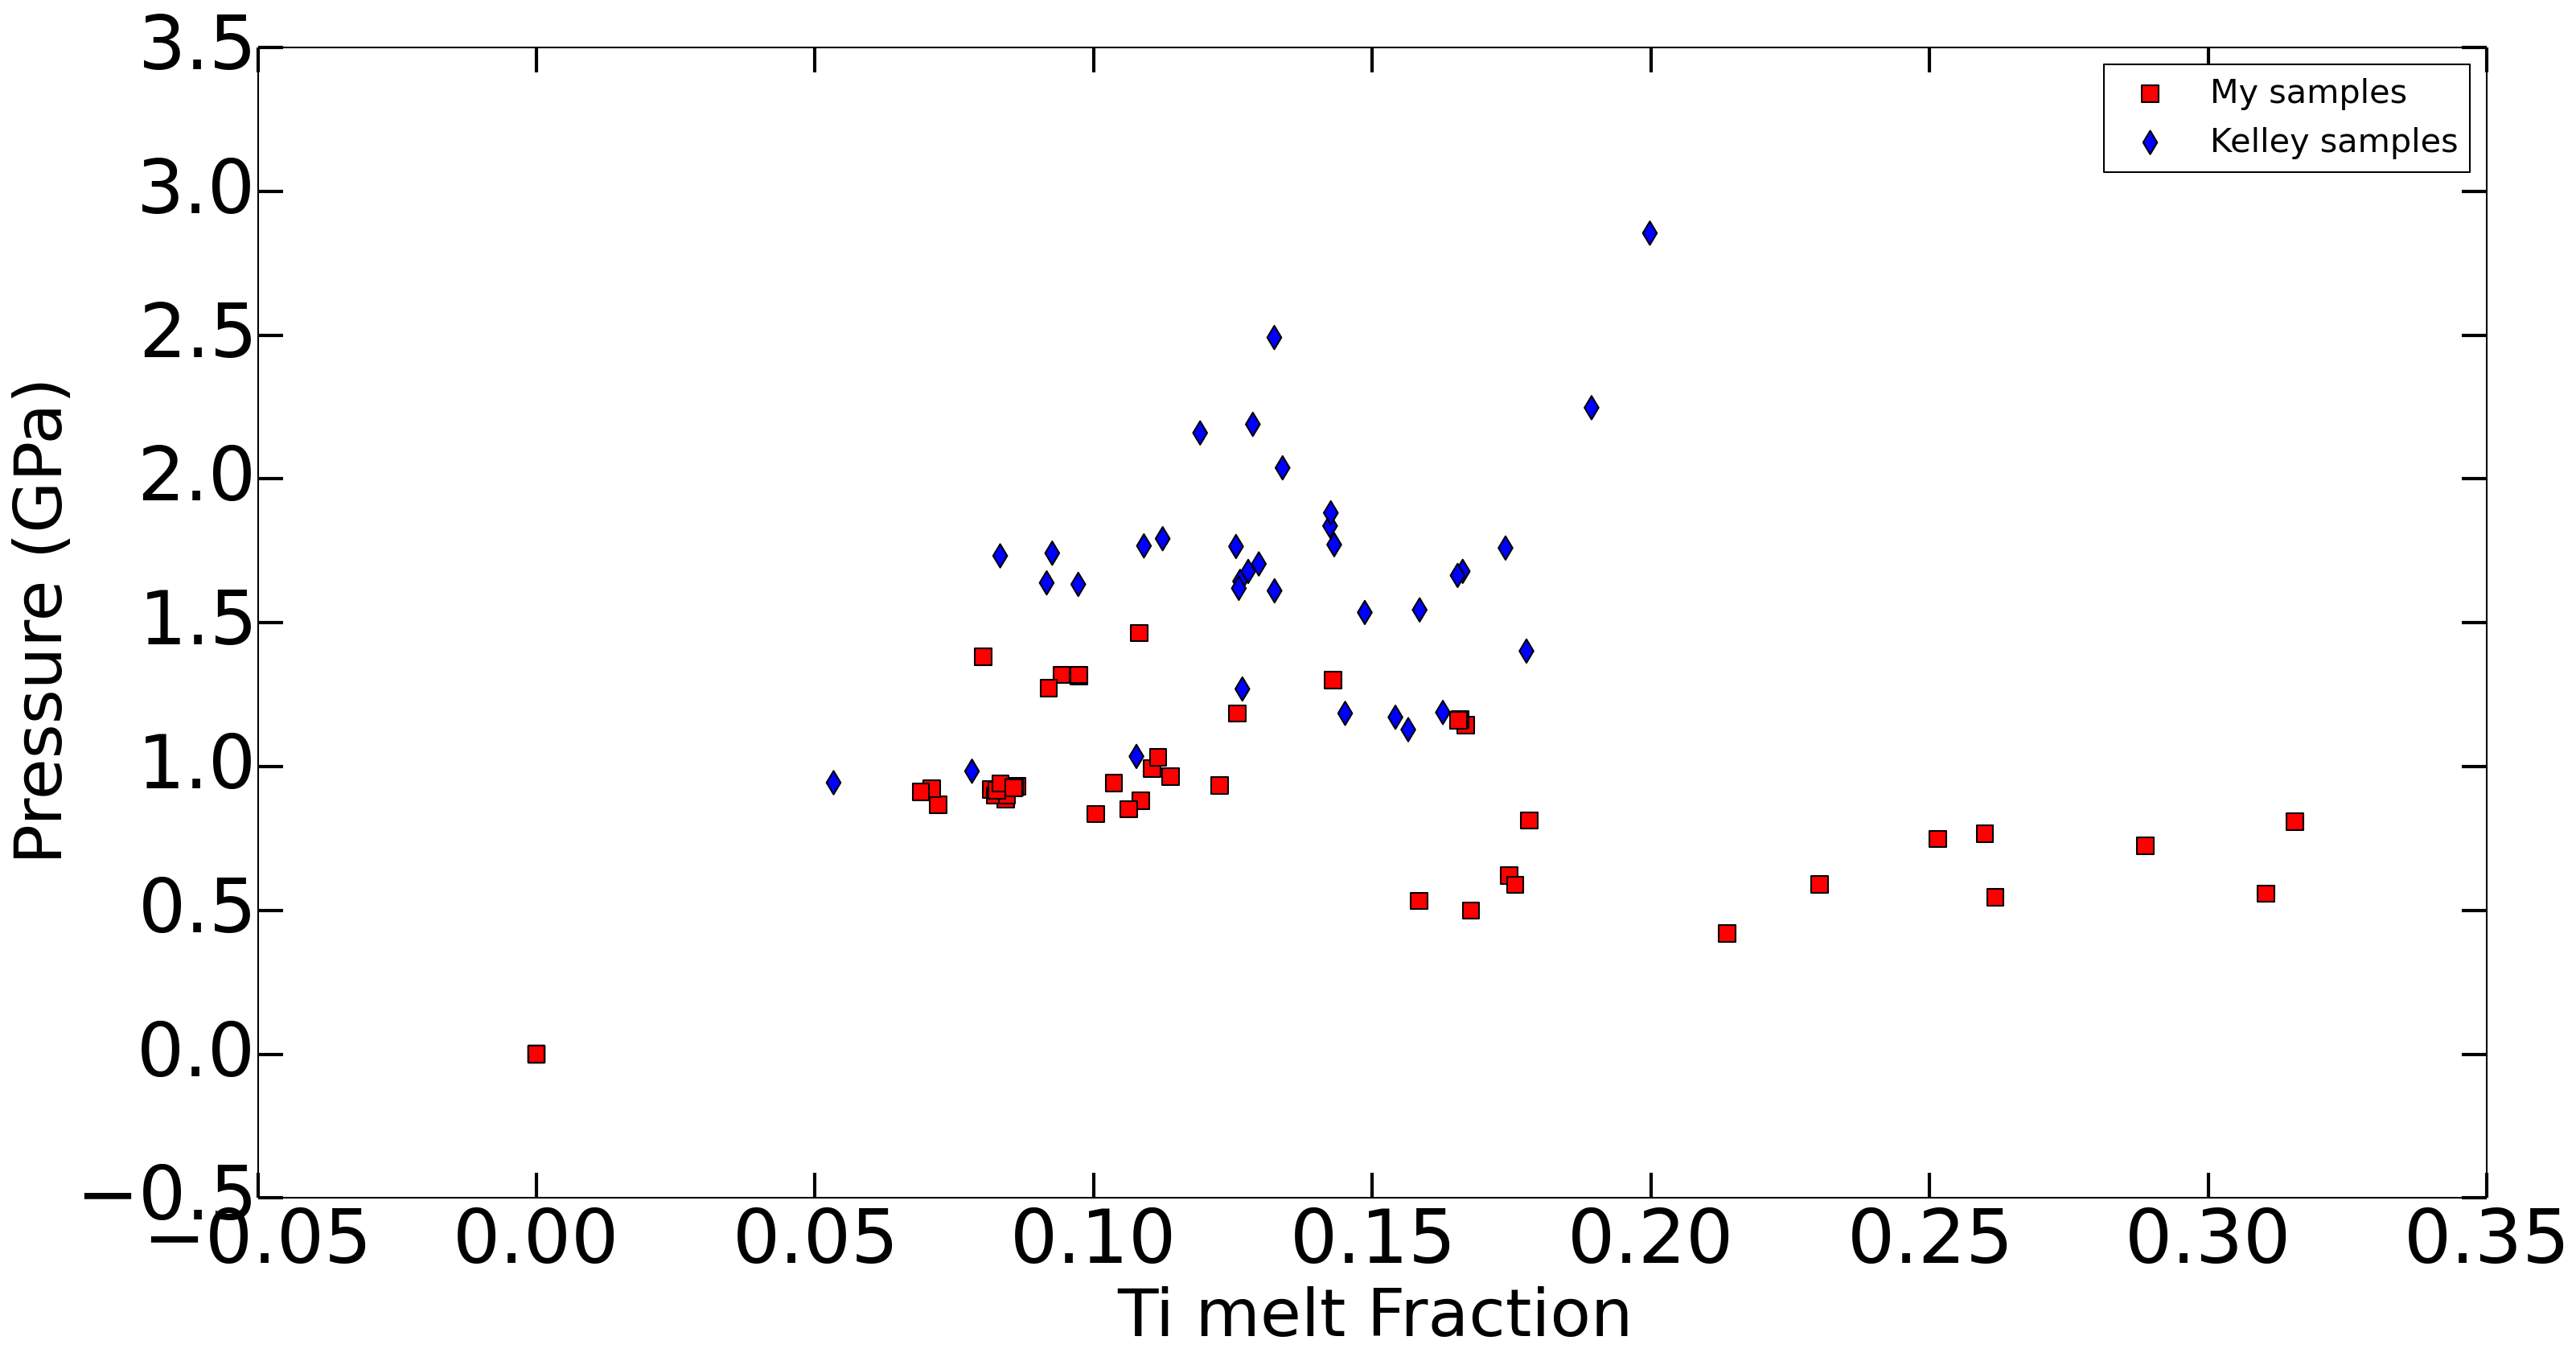
\includegraphics[width=0.9\textwidth]{/data/ap4909/30.10.2013-hot_cold_geochem/sample_testing/southern_marianas/kelley/figures/melt_fractions/mf_vs_P.png}
\label{ti_resid_v_f}
\captionsetup{singlelinecheck=off}
\caption[]{
\begin{itemize}
\item Assuming 4 wt\% H2O for our samples, 0.123wt\% mantle source Ti, 0.25 fo2.
\end{itemize}
}
\end{figure}
\begin{figure}[H]
%/data/ap4909/30.10.2013-hot_cold_geochem/sample_testing/southern_marianas/kelley/mf_vs_ti.py
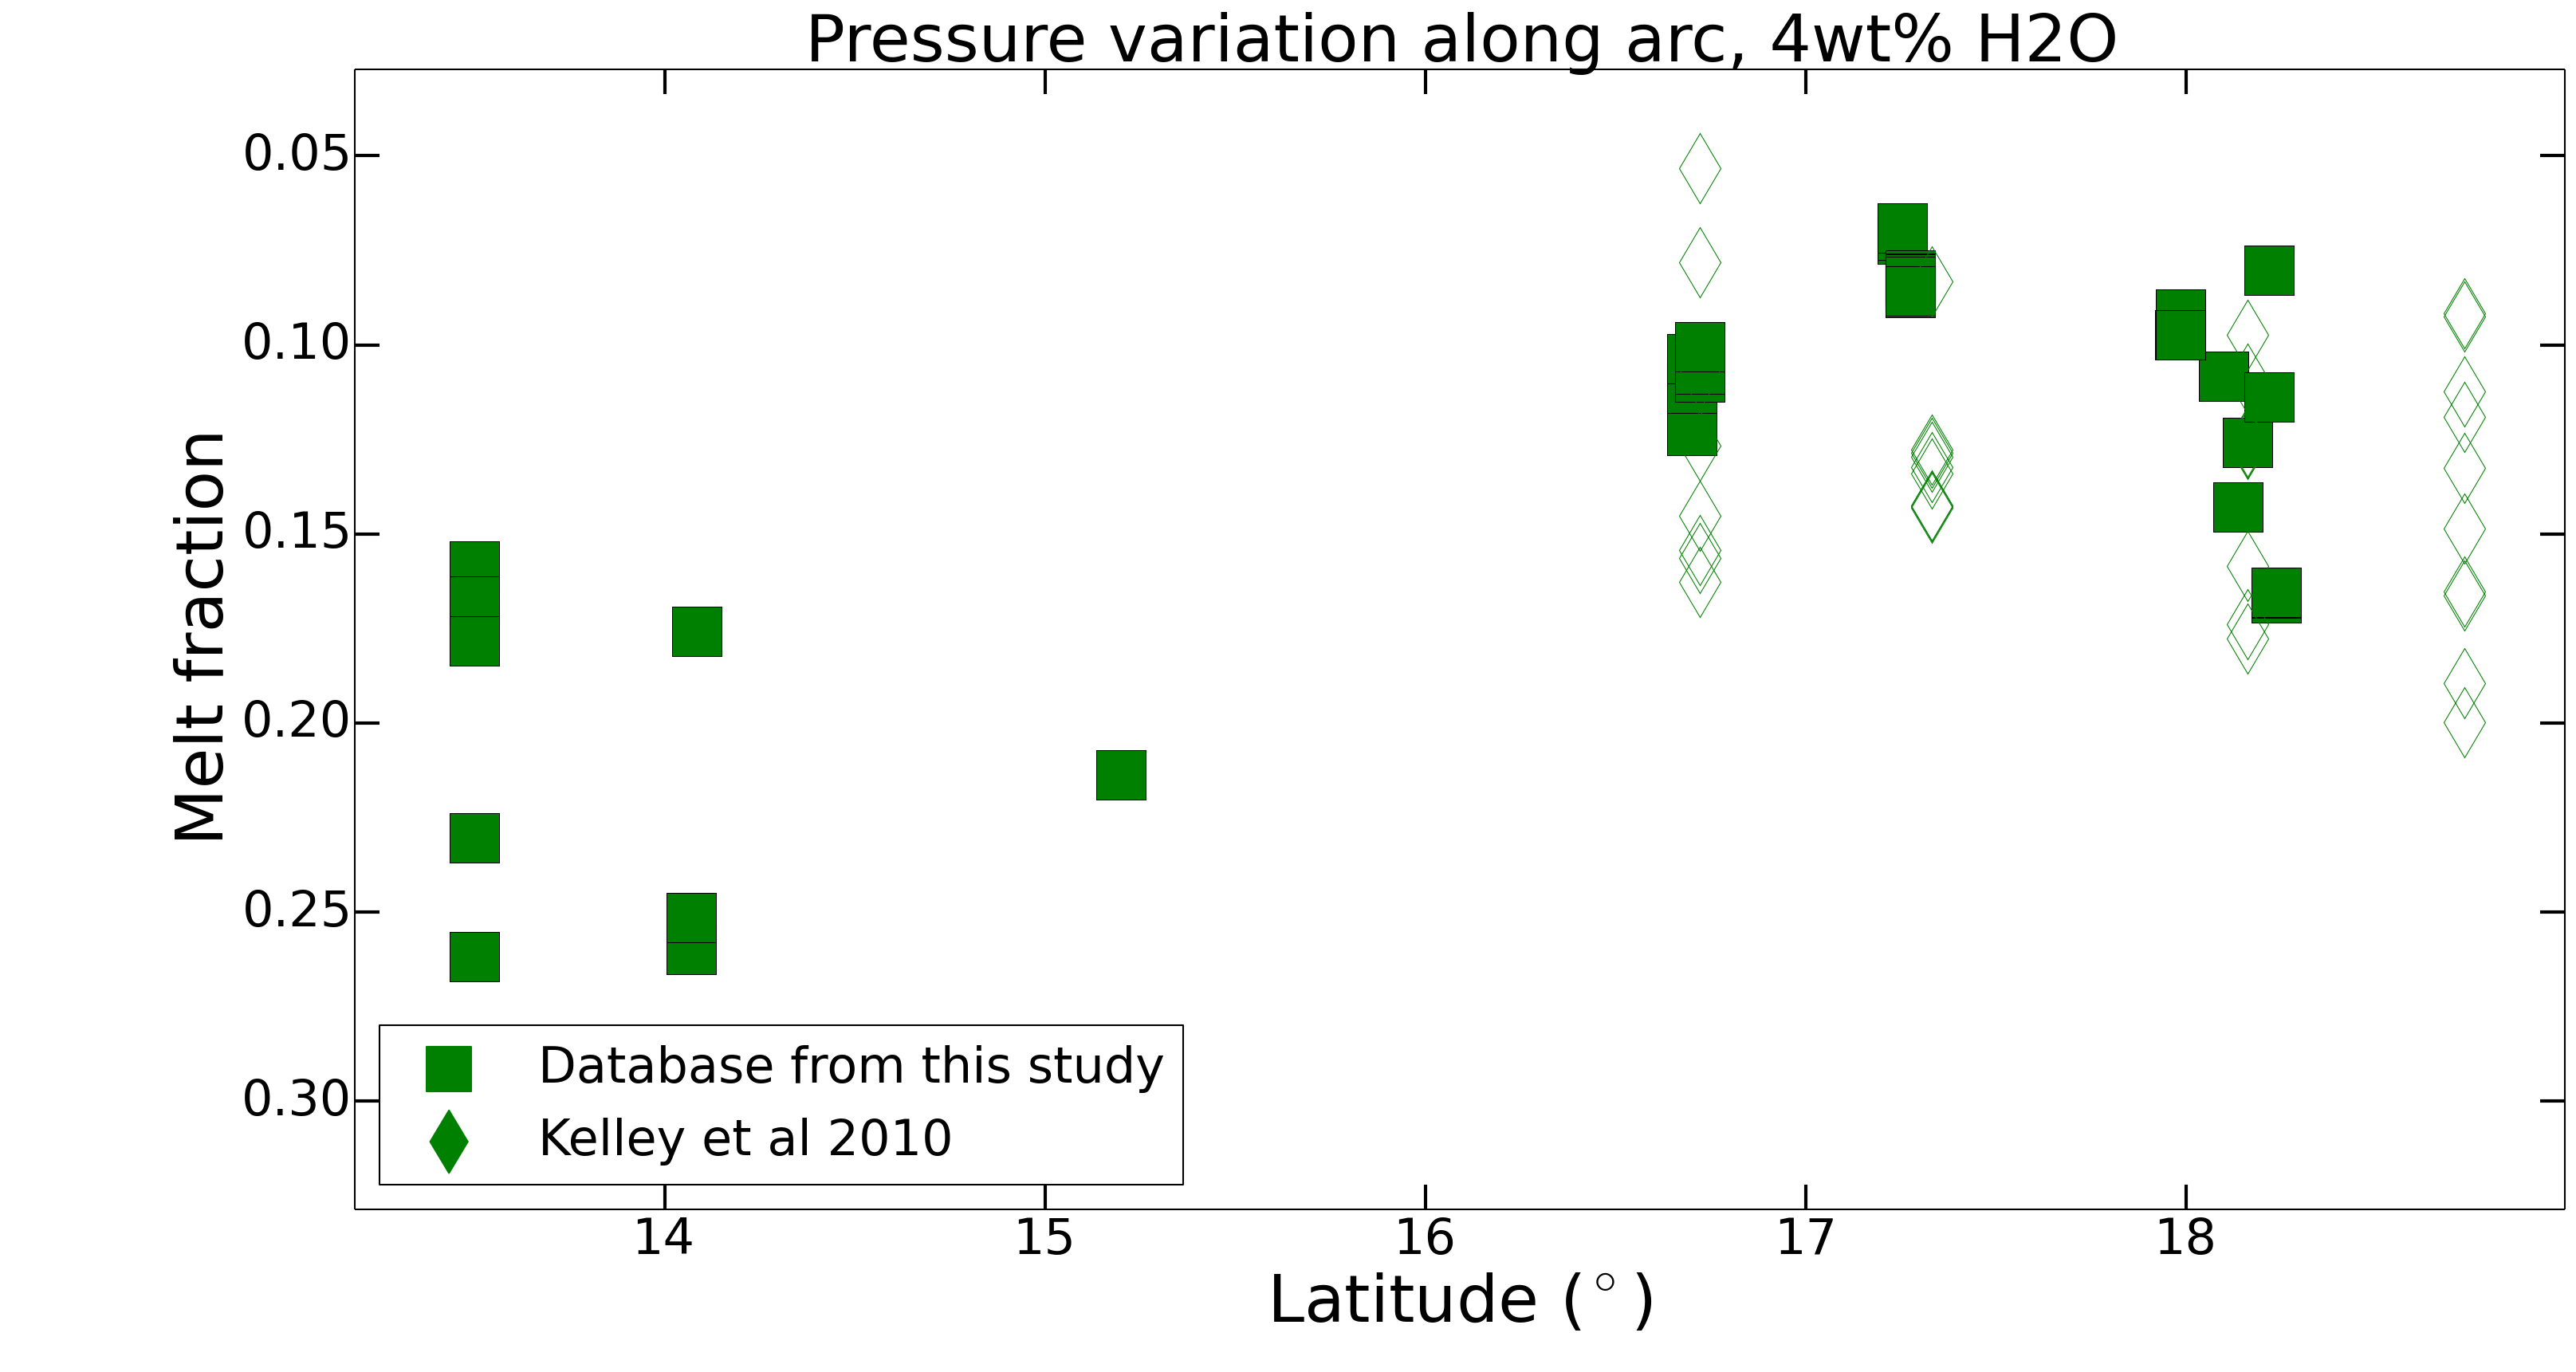
\includegraphics[width=0.9\textwidth]{/data/ap4909/30.10.2013-hot_cold_geochem/sample_testing/southern_marianas/kelley/figures/mf_vs_lat/dataset_comparison/Southern_Marianas.png}
\label{ti_resid_v_f}
\captionsetup{singlelinecheck=off}
\caption[]{
\begin{itemize}
\item Assuming 4 wt\% H2O for our samples, 0.123wt\% mantle source Ti, 0.25 fo2. 
\end{itemize}
}
\end{figure}
\begin{figure}[H]
%/data/ap4909/30.10.2013-hot_cold_geochem/sample_testing/southern_marianas/kelley/mf_vs_ti.py
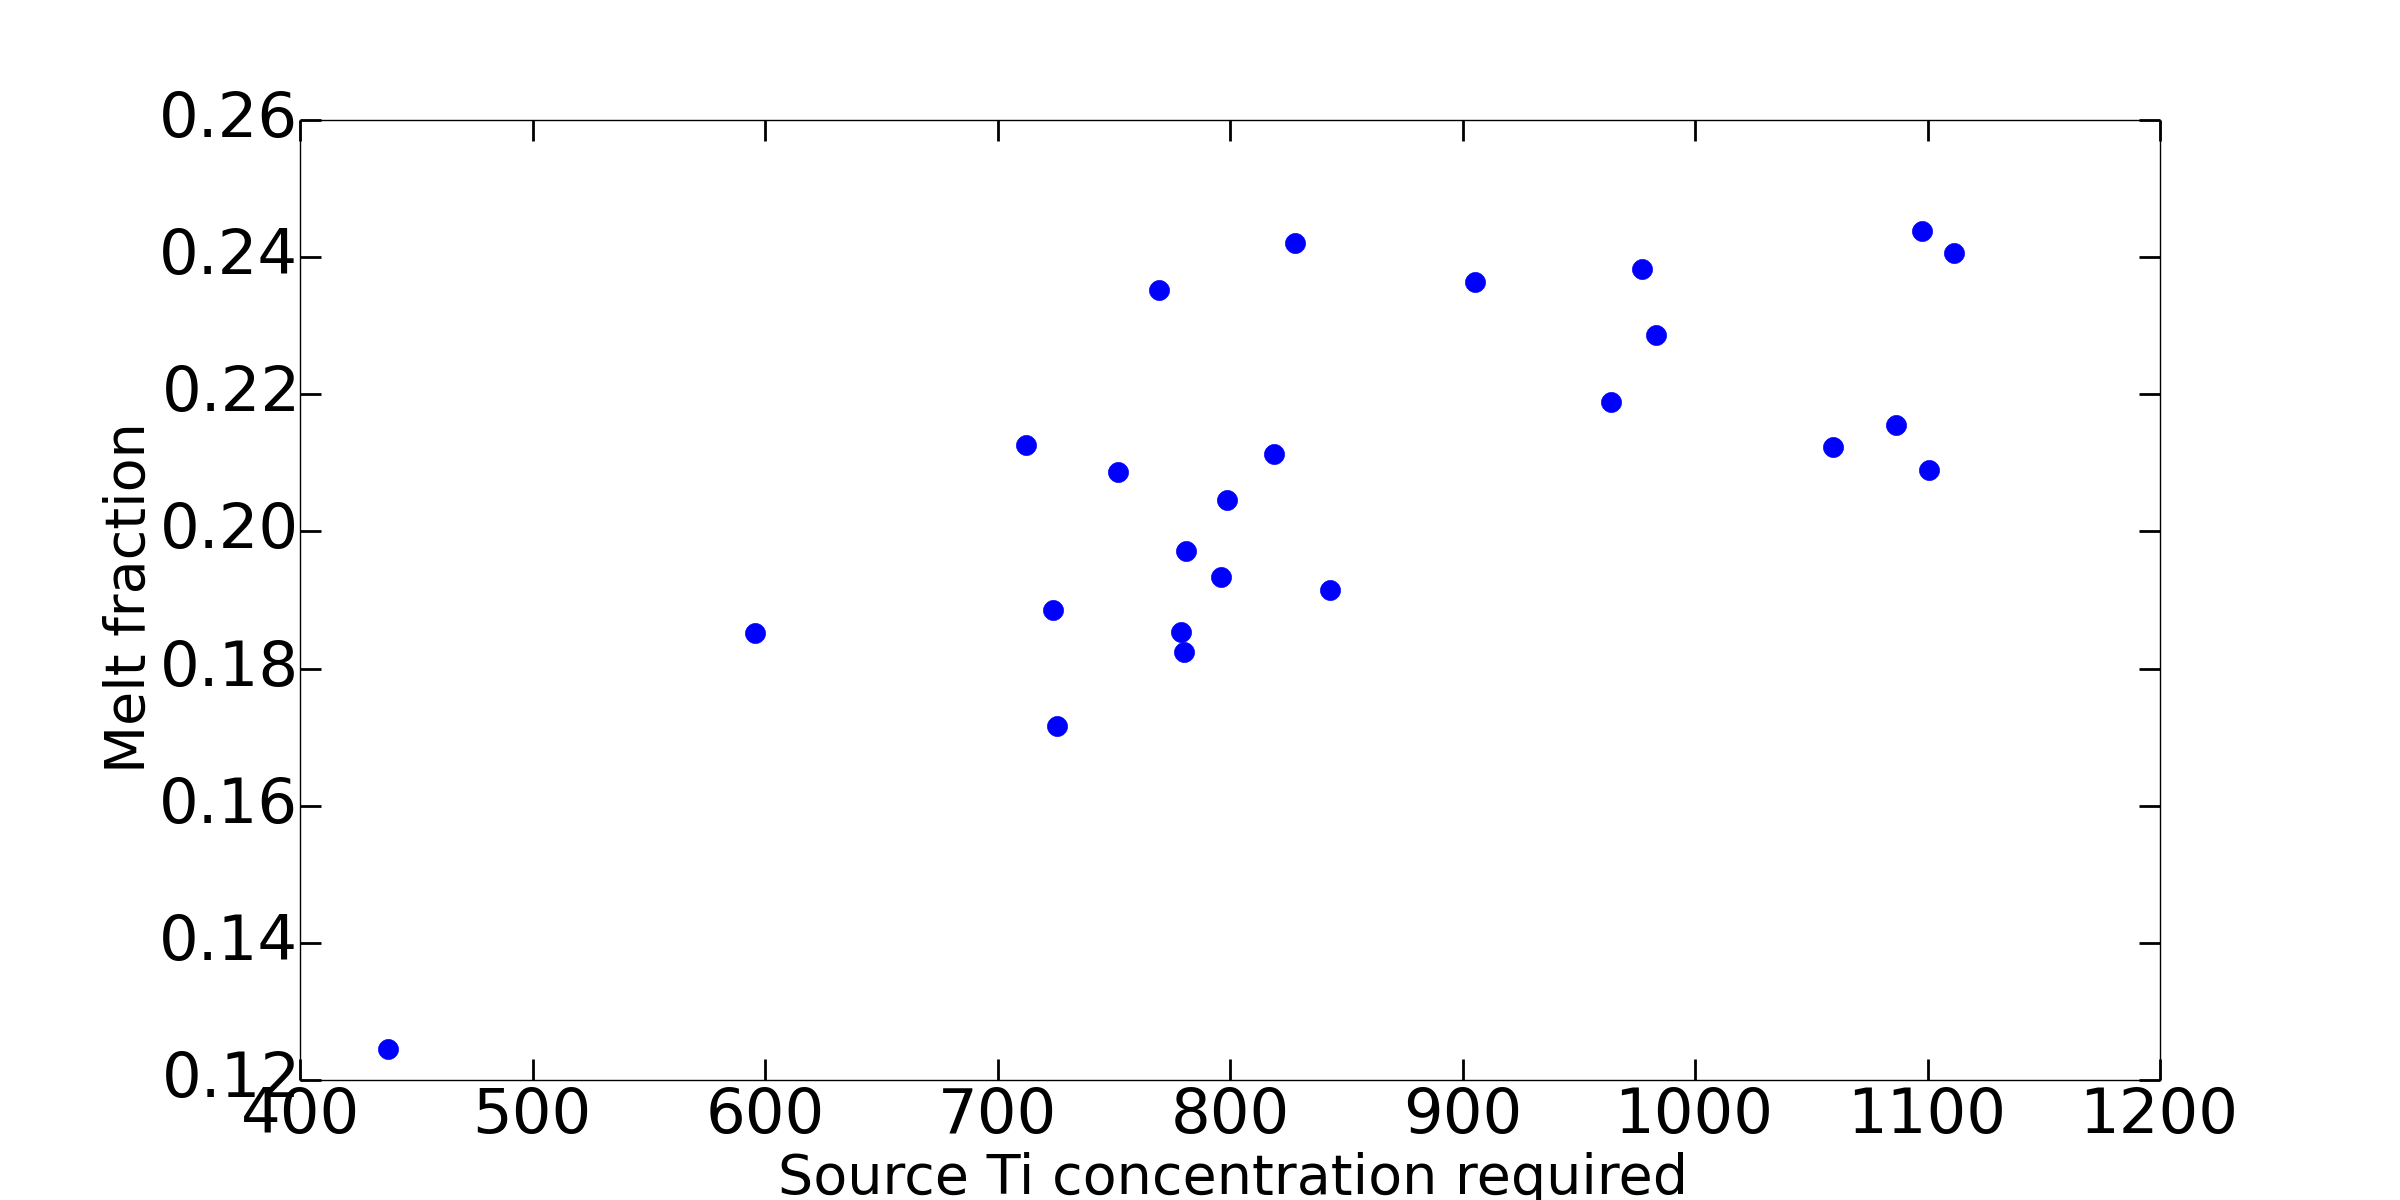
\includegraphics[width=0.9\textwidth]{/data/ap4909/30.10.2013-hot_cold_geochem/mantle_temp_cals/new_correct_mg_est/south_marianas/figures/kelley_ti_overlap/mf_vs_source_ti_required.png}
\label{ti_resid_v_f}
\captionsetup{singlelinecheck=off}
\caption[]{
\begin{itemize}
\item Assuming 4 wt\% H2O for our samples. DMM has a concentration of 713 ppm. In \cite{kelley2010mantle} they infer a source Ti of 737 ppm from TiO$_2$/Y ratios. 
\end{itemize}
}
\end{figure}

\begin{itemize}
\item Kelley correct back to Mg\#=0.9 in olivine correction.
\item In thermobarometric calculations of melt fraction assume a more refractory source. The constants they use are for a DMM1 composition, which is equivalent to a Mg\# of 0.899. After extraction of 15-25wt\% melt, the residue would actually have a Mg\# 0.91-0.92. Underestimating the Mg\# could lead to a $\sim$ 0.3-0.7 GPa shallower pressure.
\item They do not include the effect of cpx exhaustion, which is exhausted after 10\% melt extraction of DMM. Inclusion of this effect would result in a lower melt fraction as melt productivity is reduced when cpx is exhausted. Therefore \cite{kelley2010mantle} may be overestimating melt fraction when using thermobarometry. 
\end{itemize}
\begin{figure}[H]
%/data/ap4909/30.10.2013-hot_cold_geochem/sample_testing/southern_marianas/kelley/mf_vs_ti.py
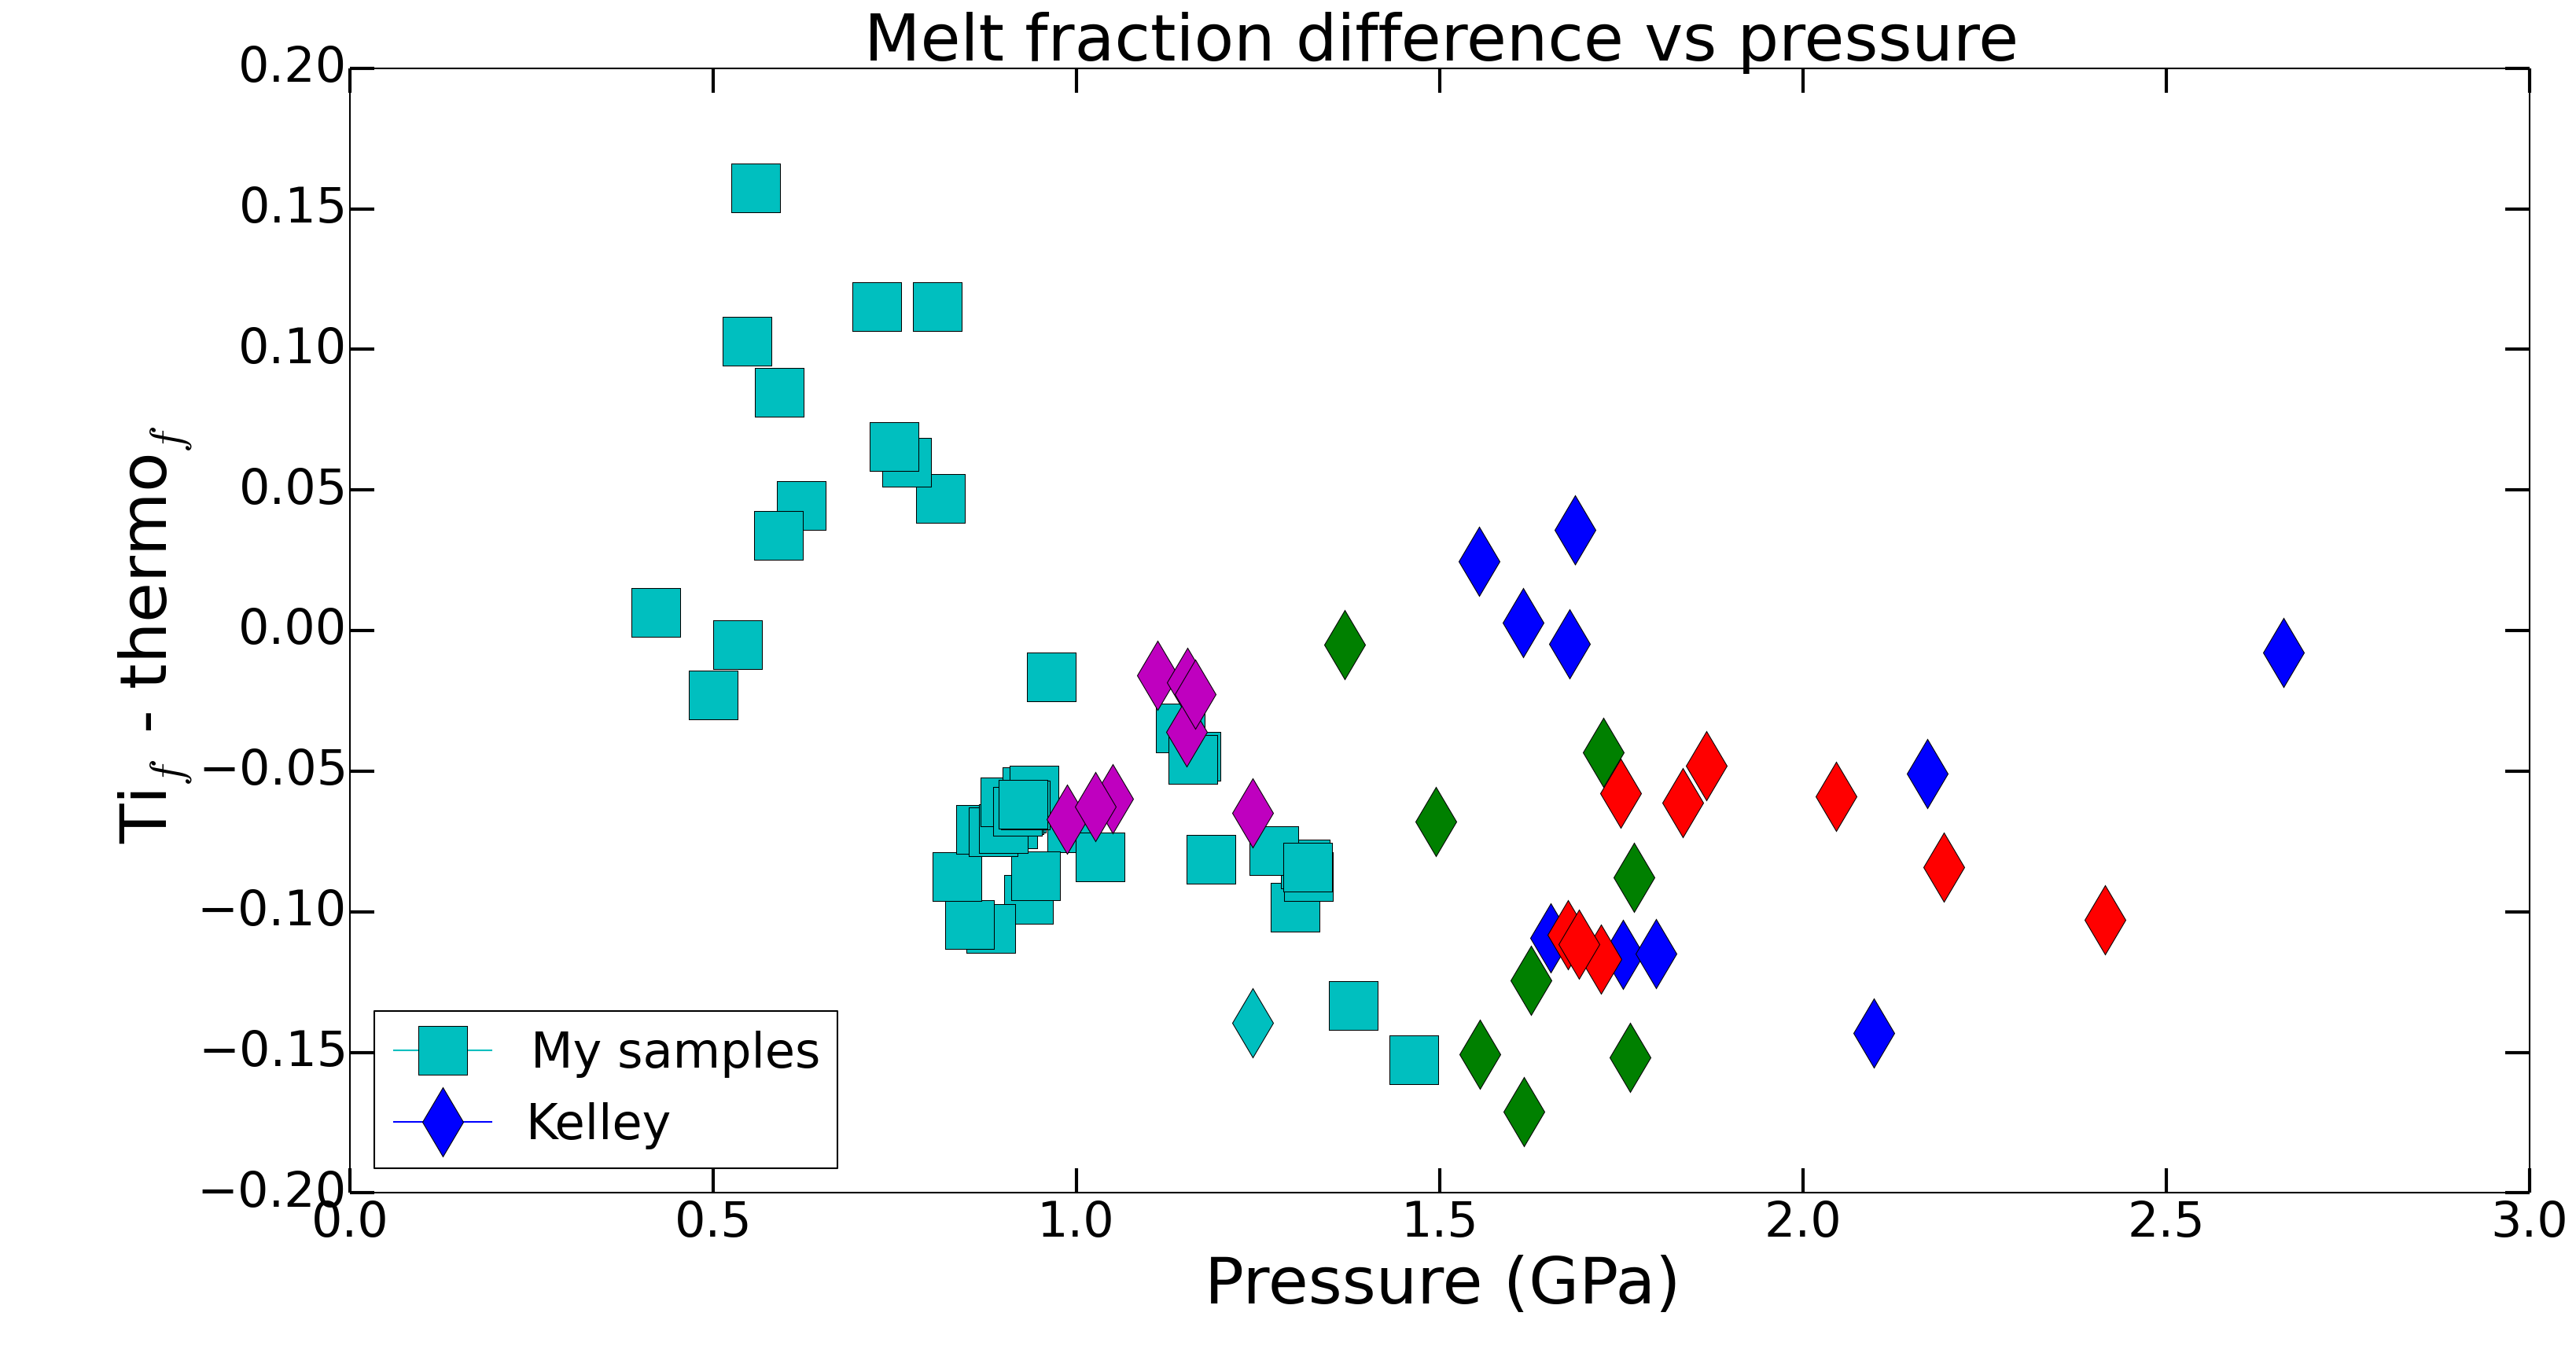
\includegraphics[width=0.9\textwidth]{/data/ap4909/30.10.2013-hot_cold_geochem/sample_testing/southern_marianas/kelley/figures/melt_fractions/mf_diff_vs_P.png}
\label{ti_resid_v_f}
\captionsetup{singlelinecheck=off}
\caption[]{
}
\end{figure}
\begin{figure}[H]
%/data/ap4909/30.10.2013-hot_cold_geochem/sample_testing/southern_marianas/kelley/mf_vs_ti.py
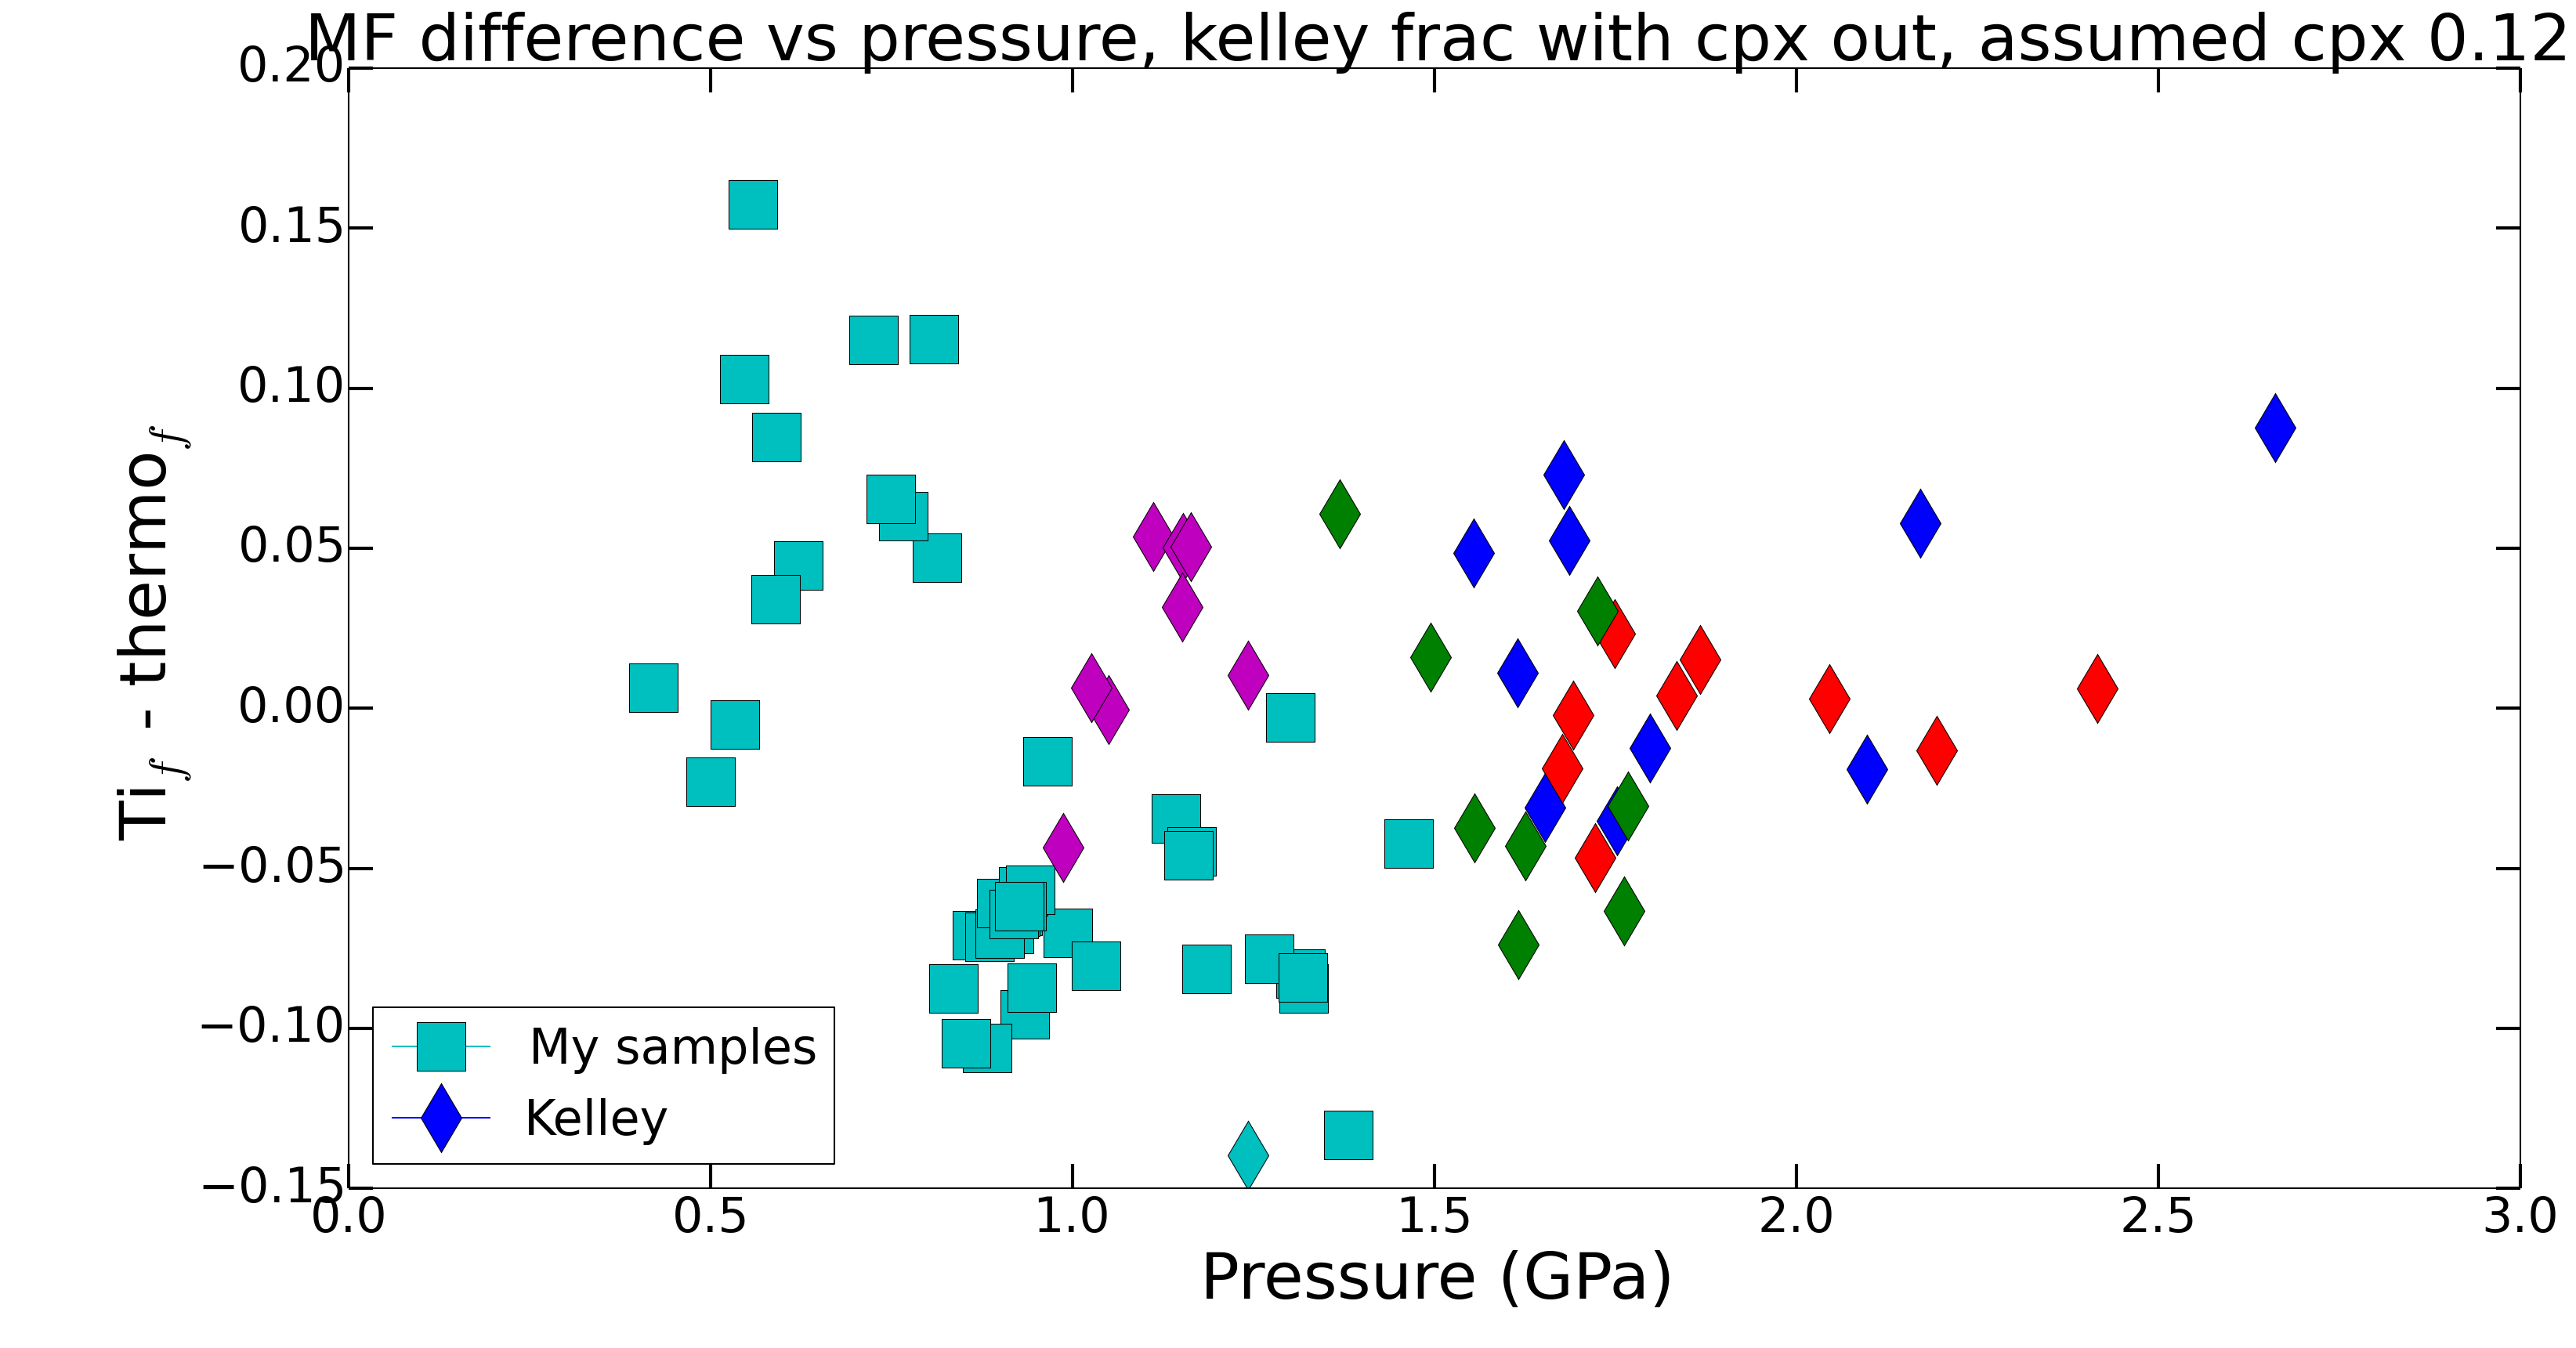
\includegraphics[width=0.9\textwidth]{/data/ap4909/30.10.2013-hot_cold_geochem/sample_testing/southern_marianas/kelley/figures/melt_fractions/mf_diff_vs_P_with_cpx_out.png}
\label{ti_resid_v_f}
\captionsetup{singlelinecheck=off}
\caption[]{

}
\end{figure}

\begin{figure}[H]
%/data/ap4909/30.10.2013-hot_cold_geochem/sample_testing/southern_marianas/kelley/mf_vs_ti.py
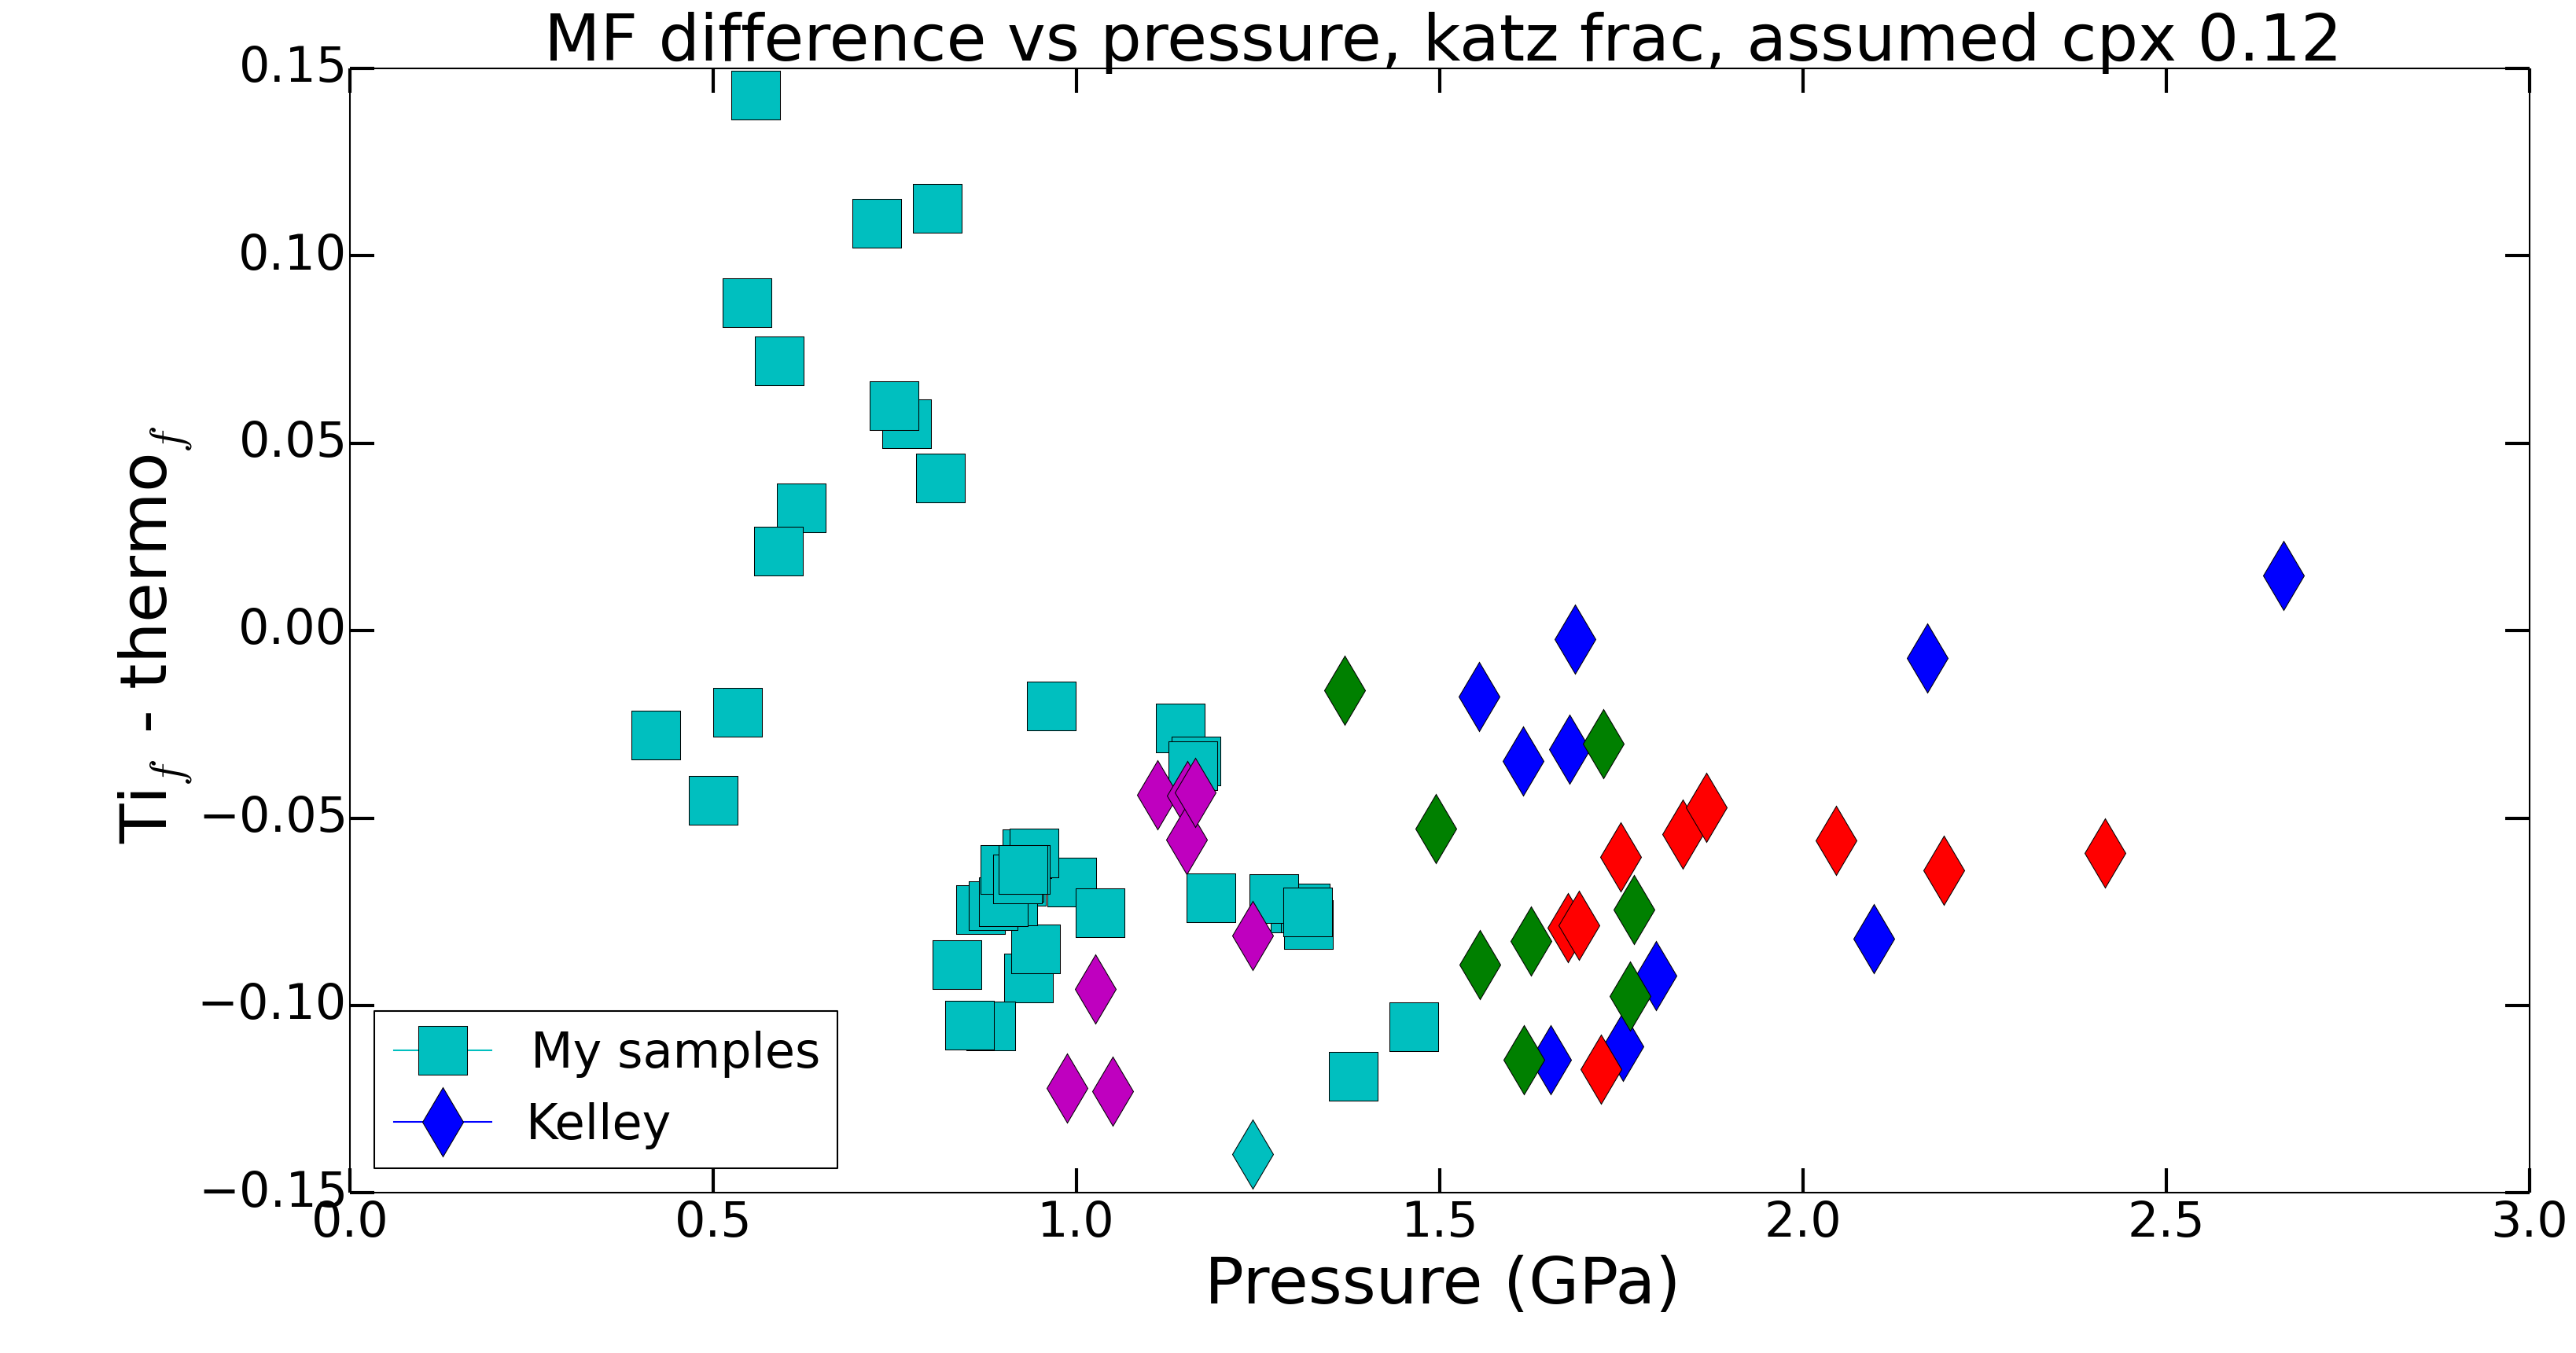
\includegraphics[width=0.9\textwidth]{/data/ap4909/30.10.2013-hot_cold_geochem/sample_testing/southern_marianas/kelley/figures/melt_fractions/katz_mf_diff_vs_P_with_cpx_out.png}
\label{ti_resid_v_f}
\captionsetup{singlelinecheck=off}
\caption[]{

}
\end{figure}
\begin{figure}[H]
%/data/ap4909/30.10.2013-hot_cold_geochem/sample_testing/southern_marianas/kelley/mf_vs_ti.py
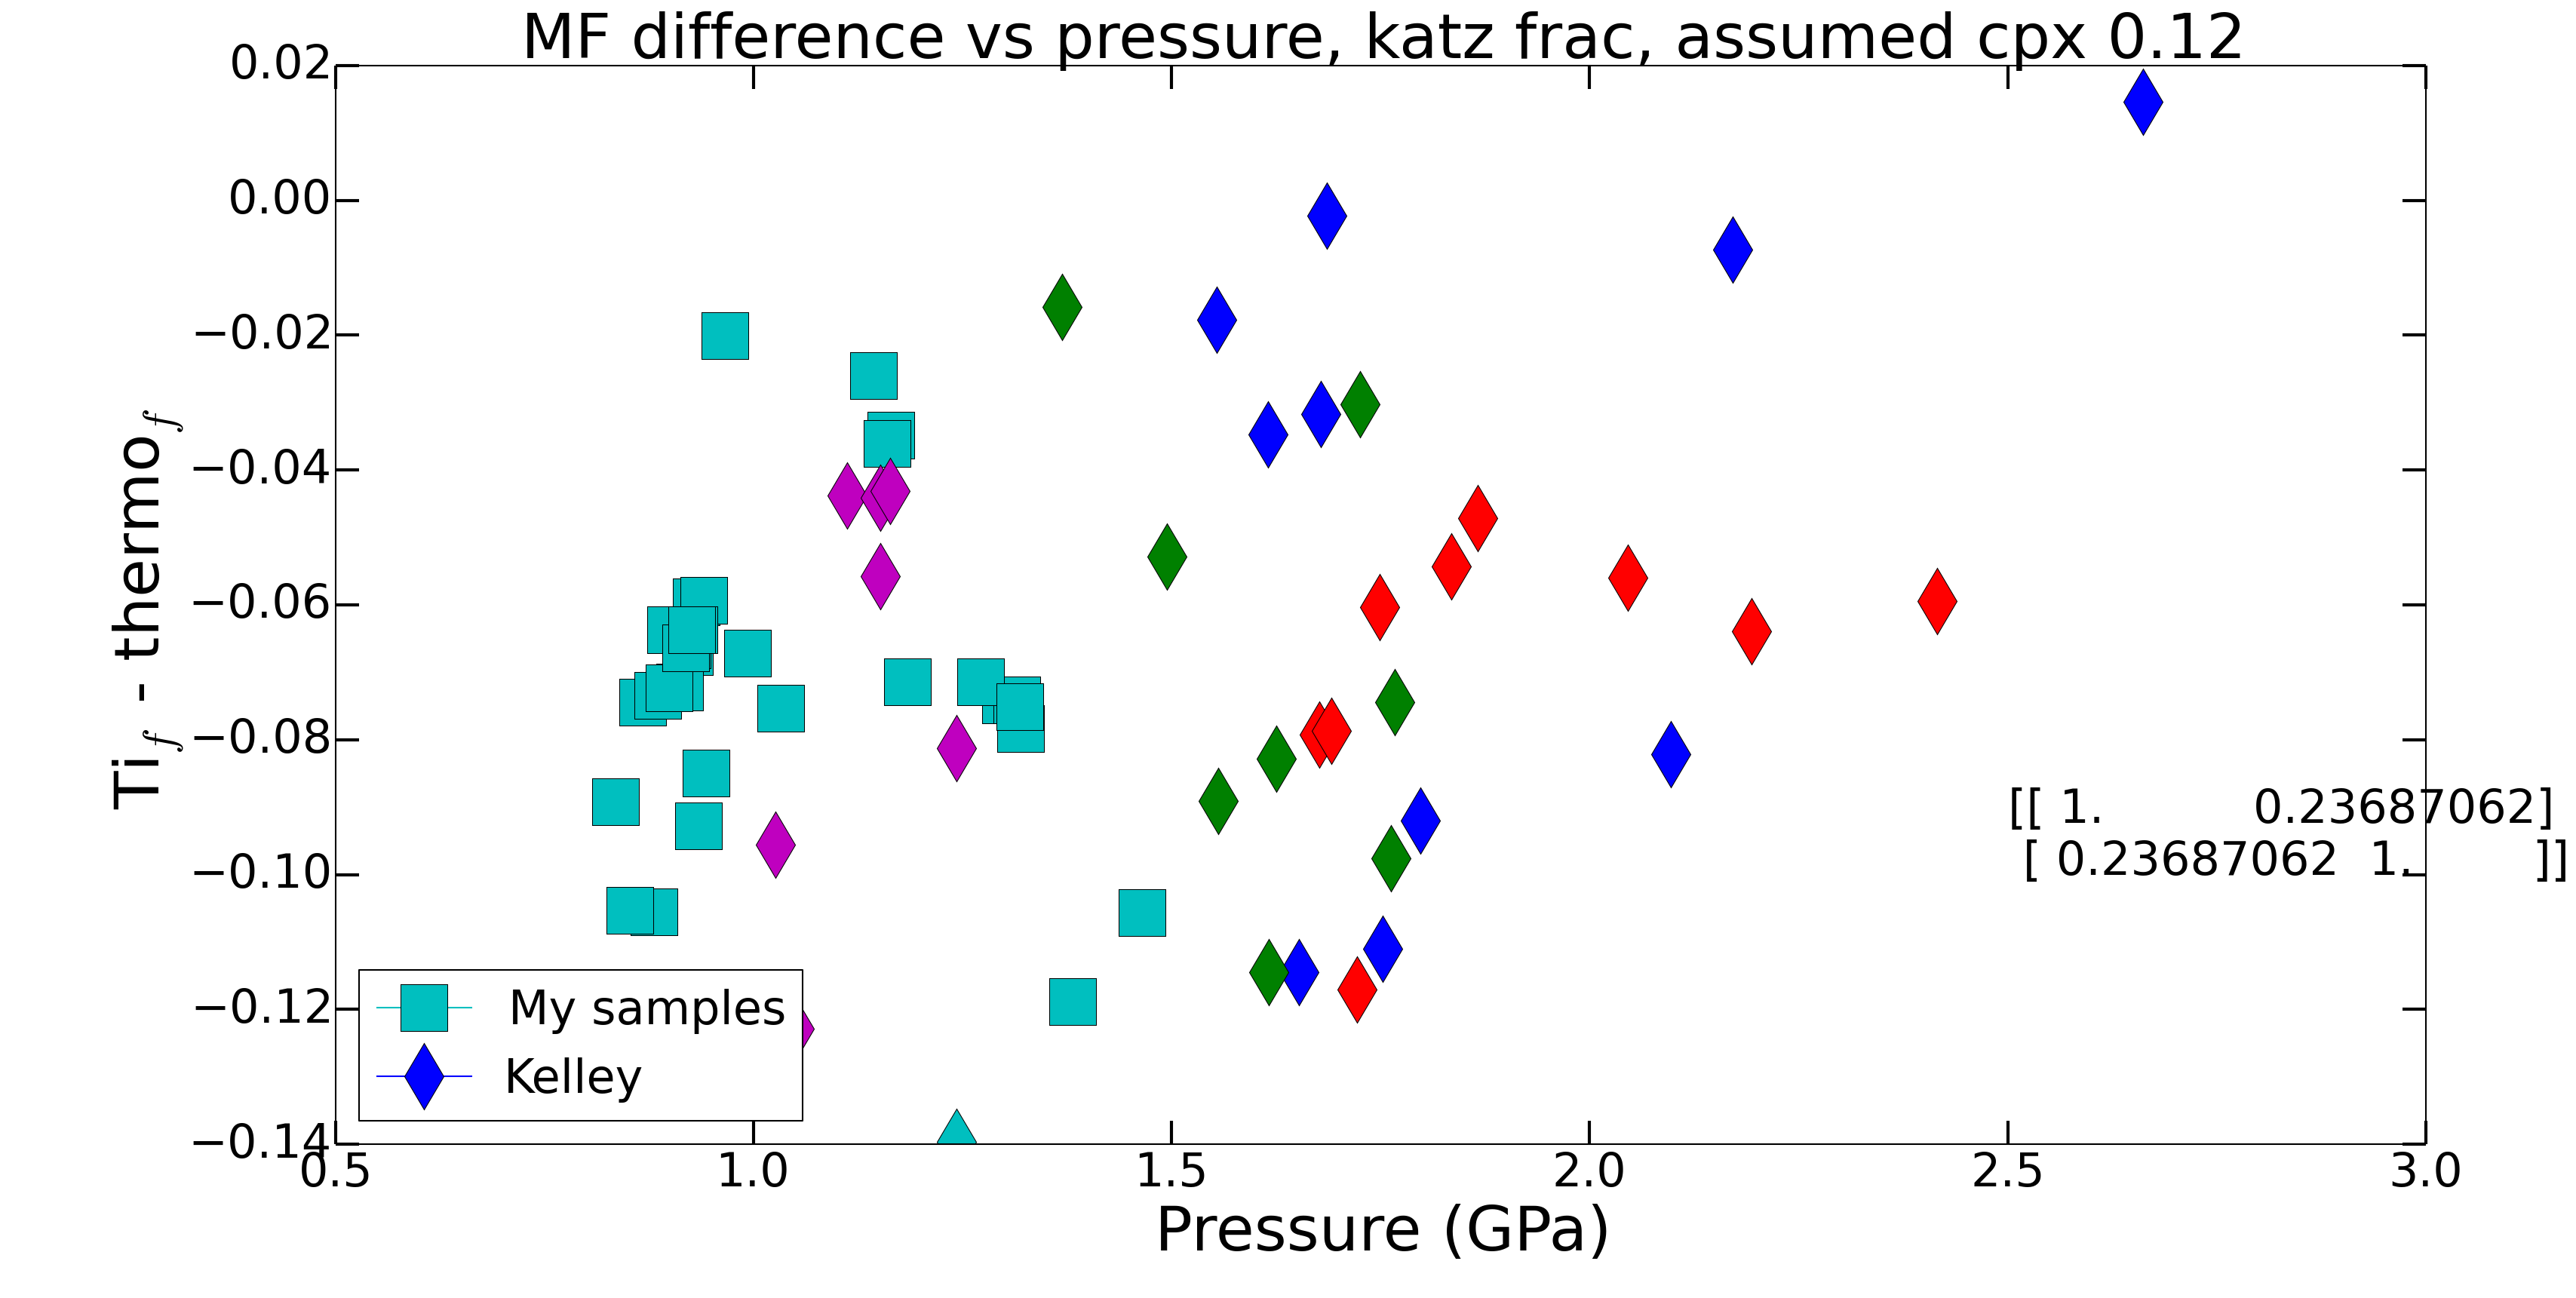
\includegraphics[width=0.9\textwidth]{/data/ap4909/30.10.2013-hot_cold_geochem/sample_testing/southern_marianas/kelley/figures/melt_fractions/katz_mf_diff_vs_P_with_cpx_out_without_southern_samples.png}
\label{ti_resid_v_f}
\captionsetup{singlelinecheck=off}
\caption[]{

}
\end{figure}
\begin{figure}[H]
%/data/ap4909/30.10.2013-hot_cold_geochem/sample_testing/southern_marianas/kelley/mf_vs_ti.py
\includegraphi
cs[width=0.9\textwidth]{/data/ap4909/30.10.2013-hot_cold_geochem/sample_testing/southern_marianas/kelley/figures/melt_fractions/thermo_mf_vs_P_katz_comparison.png}
\label{ti_resid_v_f}
\captionsetup{singlelinecheck=off}
\caption[]{
\begin{itemize}
\item Hollow symbols- Katz melt fraction.
\end{itemize}
}
\end{figure}
\begin{figure}[H]
%/data/ap4909/30.10.2013-hot_cold_geochem/sample_testing/southern_marianas/kelley/mf_vs_ti.py
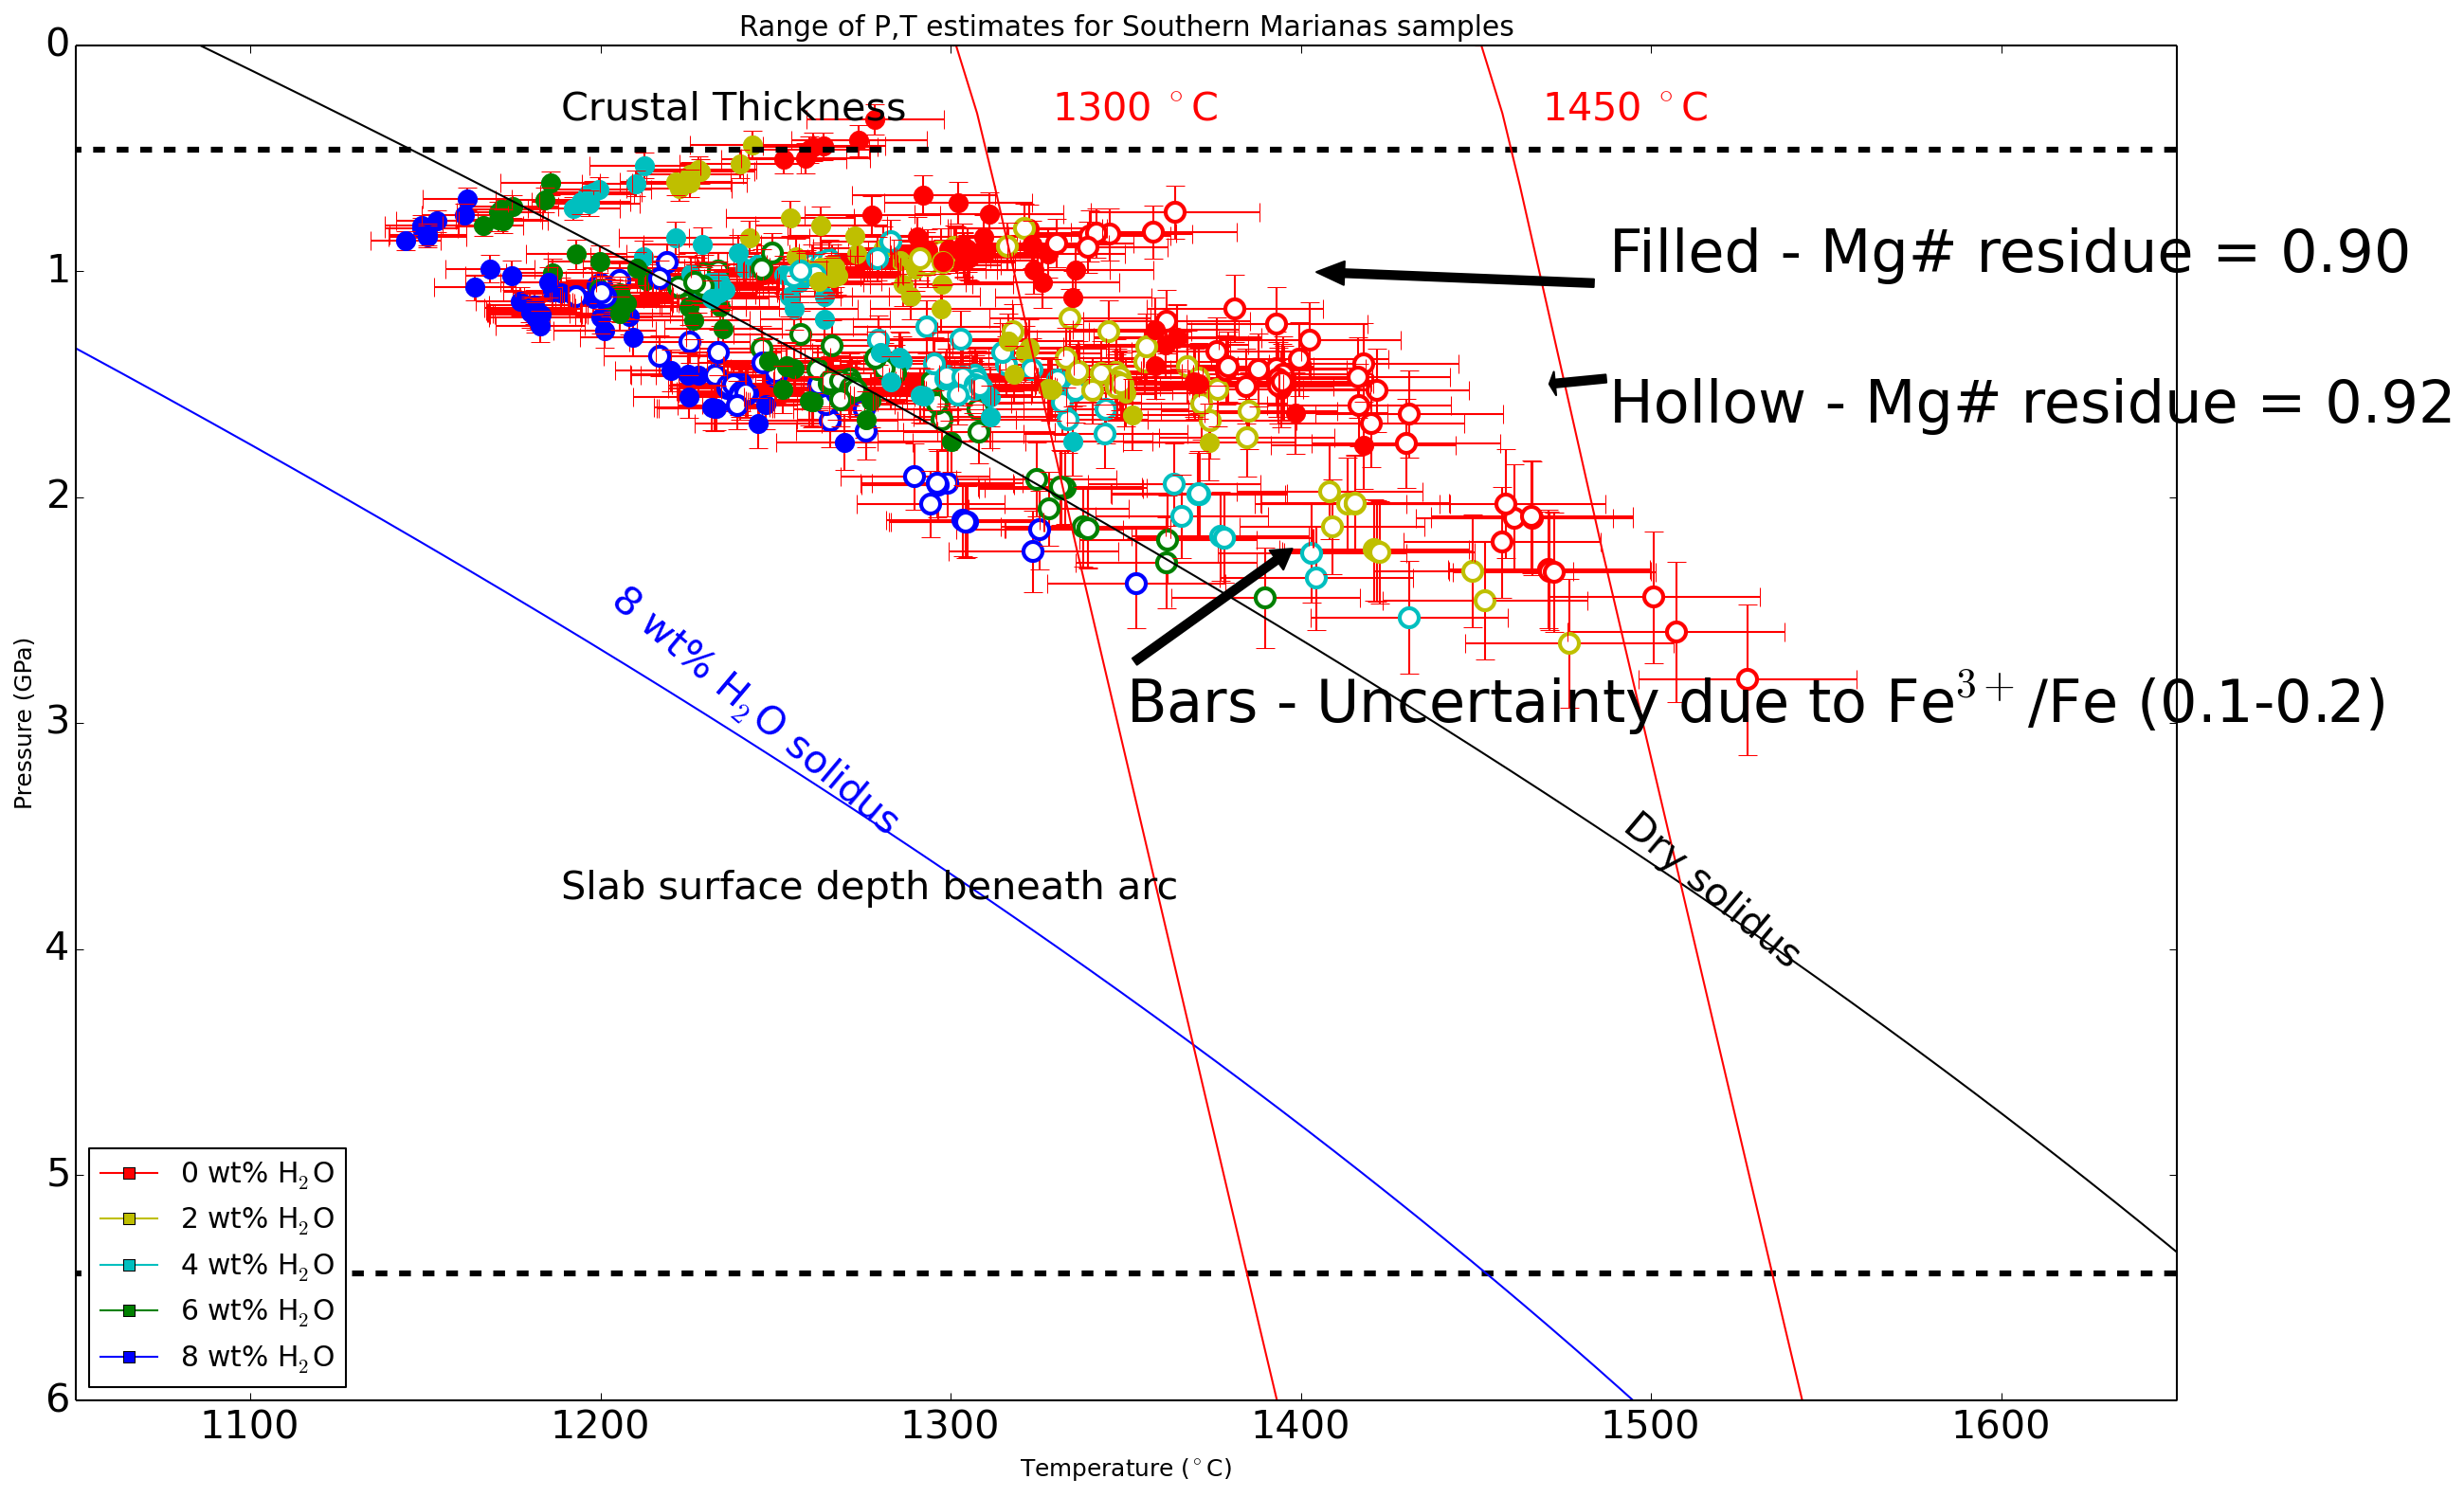
\includegraphics[width=0.9\textwidth]{/data/ap4909/30.10.2013-hot_cold_geochem/sample_testing/southern_marianas/kelley/figures/h2o_evaluation_Southern_Marianas.png}
\label{ti_resid_v_f}
\captionsetup{singlelinecheck=off}
\caption[]{

}
\end{figure}
\begin{figure}[H]
%/data/ap4909/30.10.2013-hot_cold_geochem/sample_testing/southern_marianas/kelley/mf_vs_ti.py
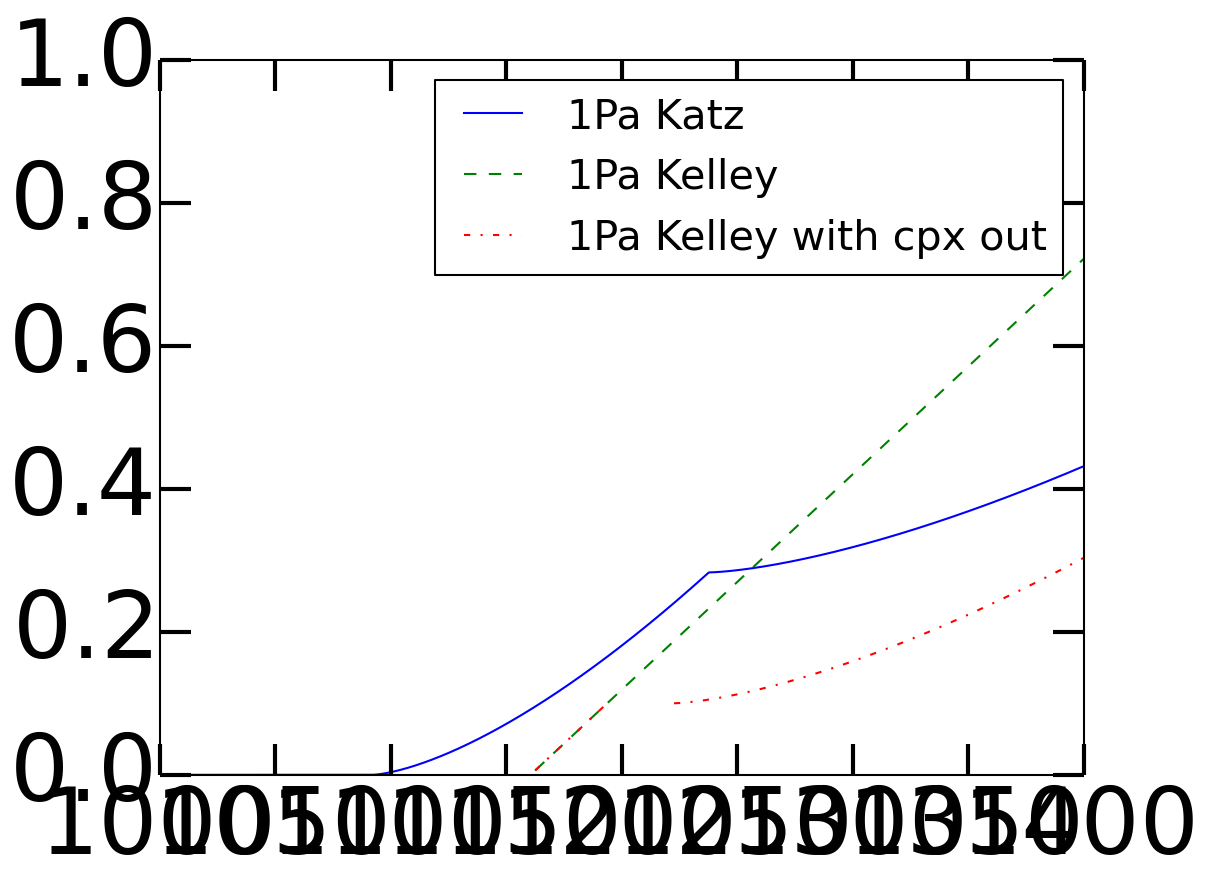
\includegraphics[width=0.9\textwidth]{/data/ap4909/30.10.2013-hot_cold_geochem/sample_testing/southern_marianas/kelley/figures/katz_kelley_base_comparison.png}
\label{ti_resid_v_f}
\captionsetup{singlelinecheck=off}
\caption[]{

}
\end{figure}

\begin{figure}[H]
%/data/ap4909/30.10.2013-hot_cold_geochem/sample_testing/southern_marianas/kelley/mf_vs_ti.py
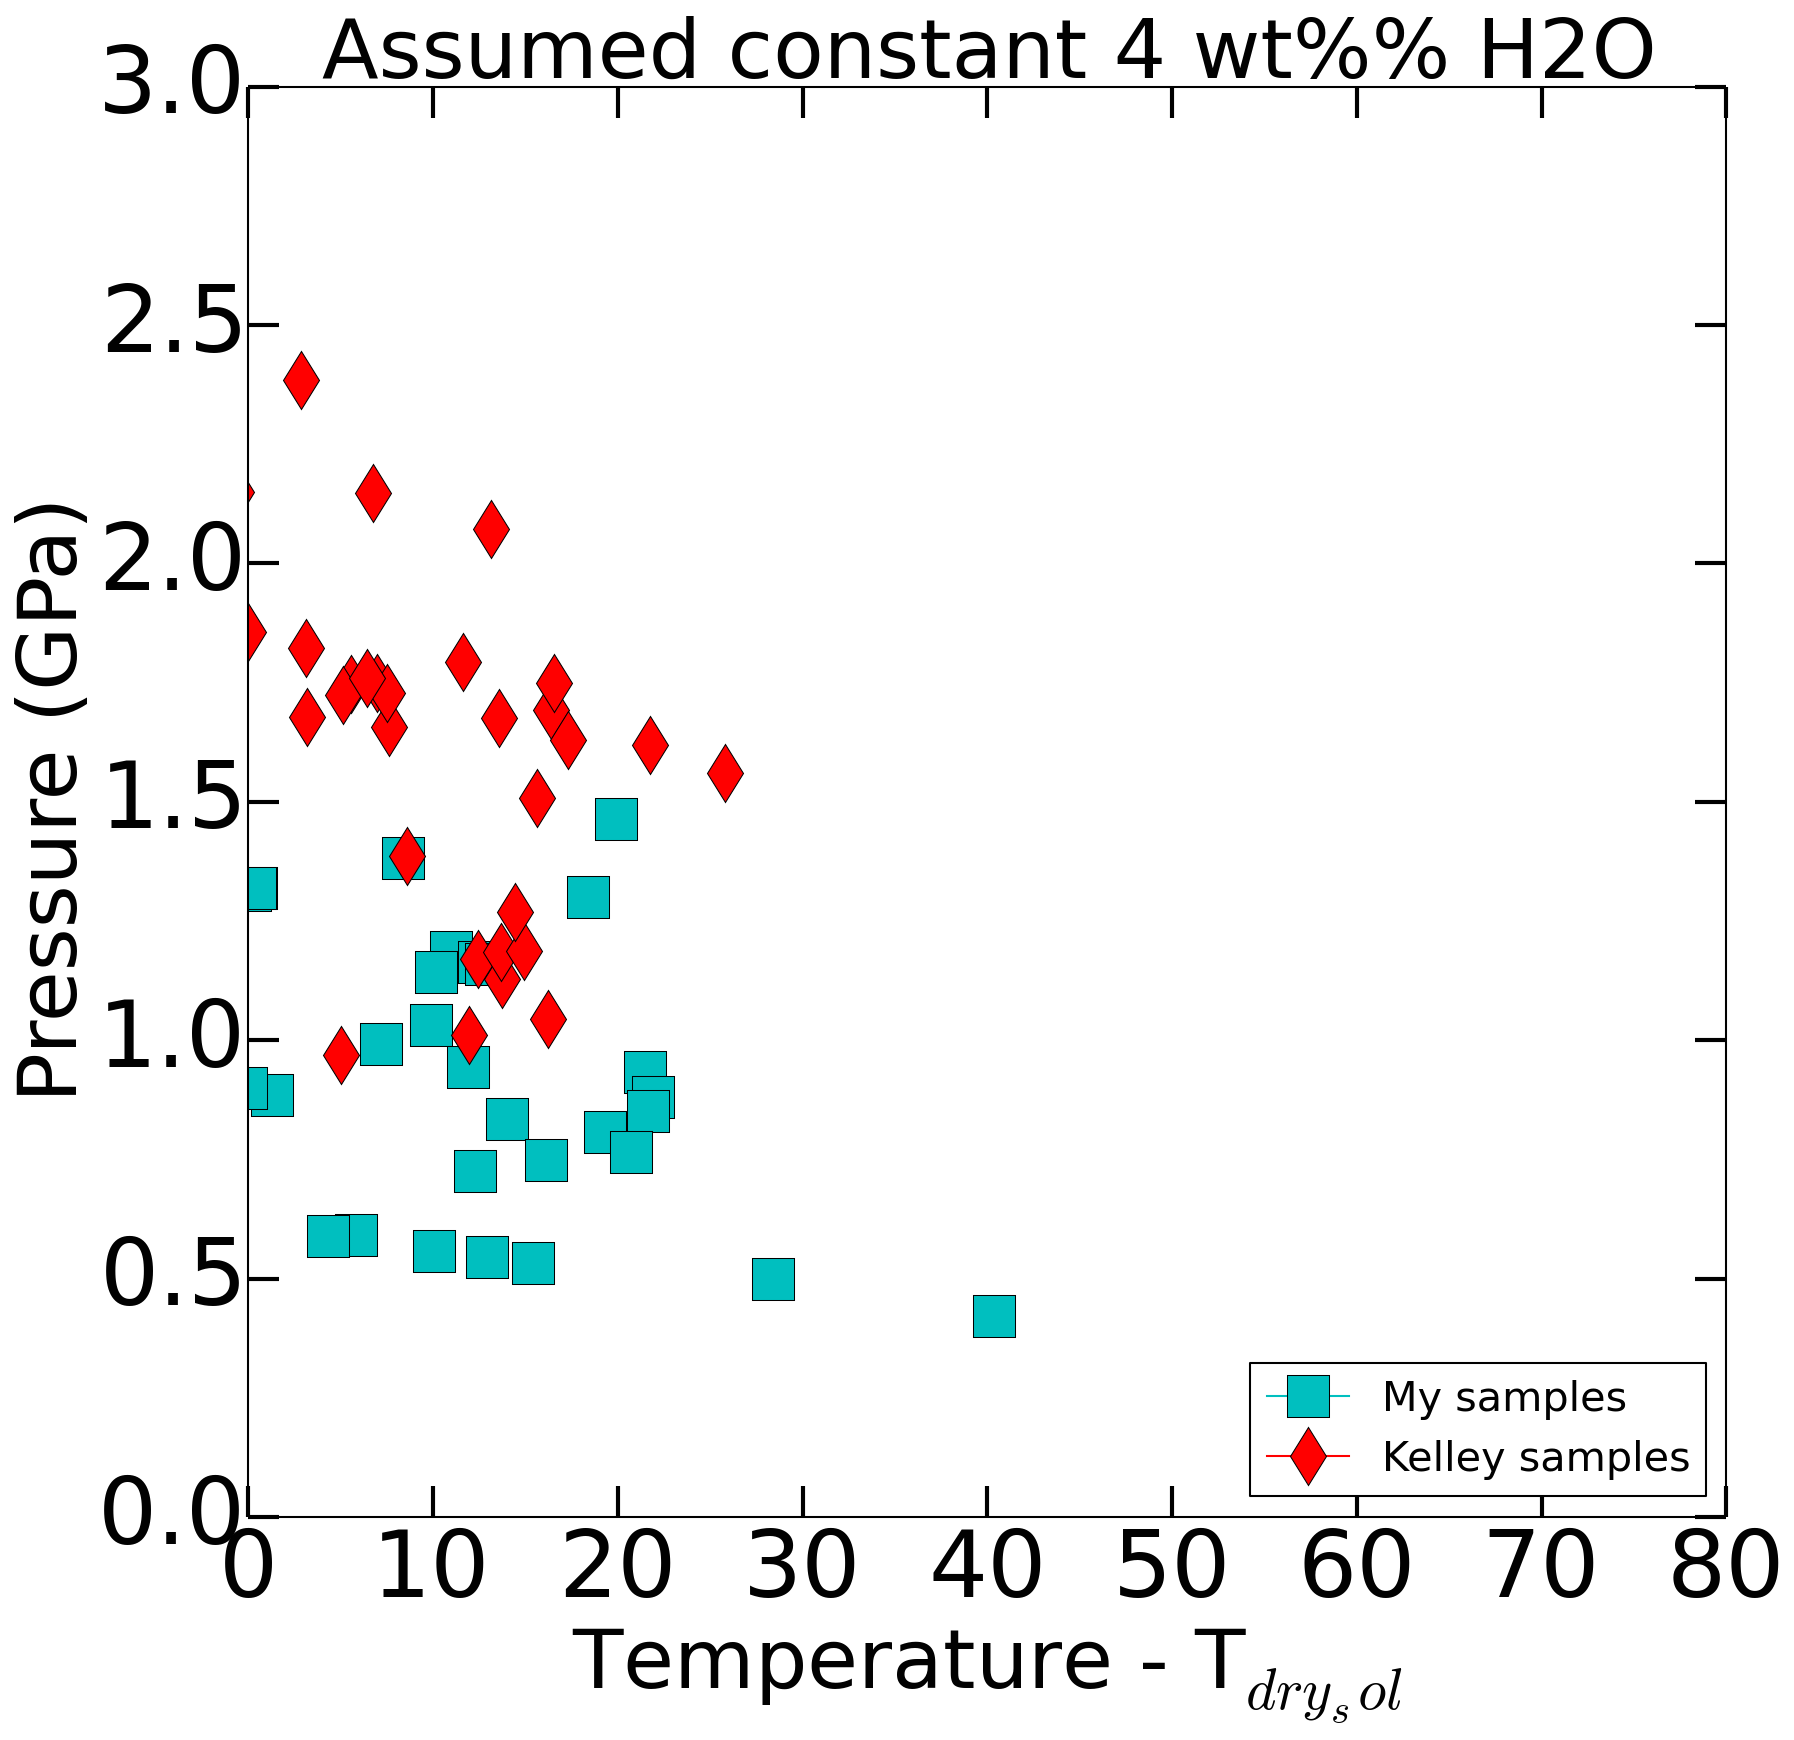
\includegraphics[width=0.9\textwidth]{/data/ap4909/30.10.2013-hot_cold_geochem/sample_testing/southern_marianas/kelley/figures/t_minus_t_dry_sol_vs_P.png}
\label{ti_resid_v_f}
\captionsetup{singlelinecheck=off}
\caption[]{

}
\end{figure}

\section{Katz/Kelley comparison}
\begin{figure}[H]
%/data/ap4909/30.10.2013-hot_cold_geochem/sample_testing/southern_marianas/kelley/mf_vs_ti.py
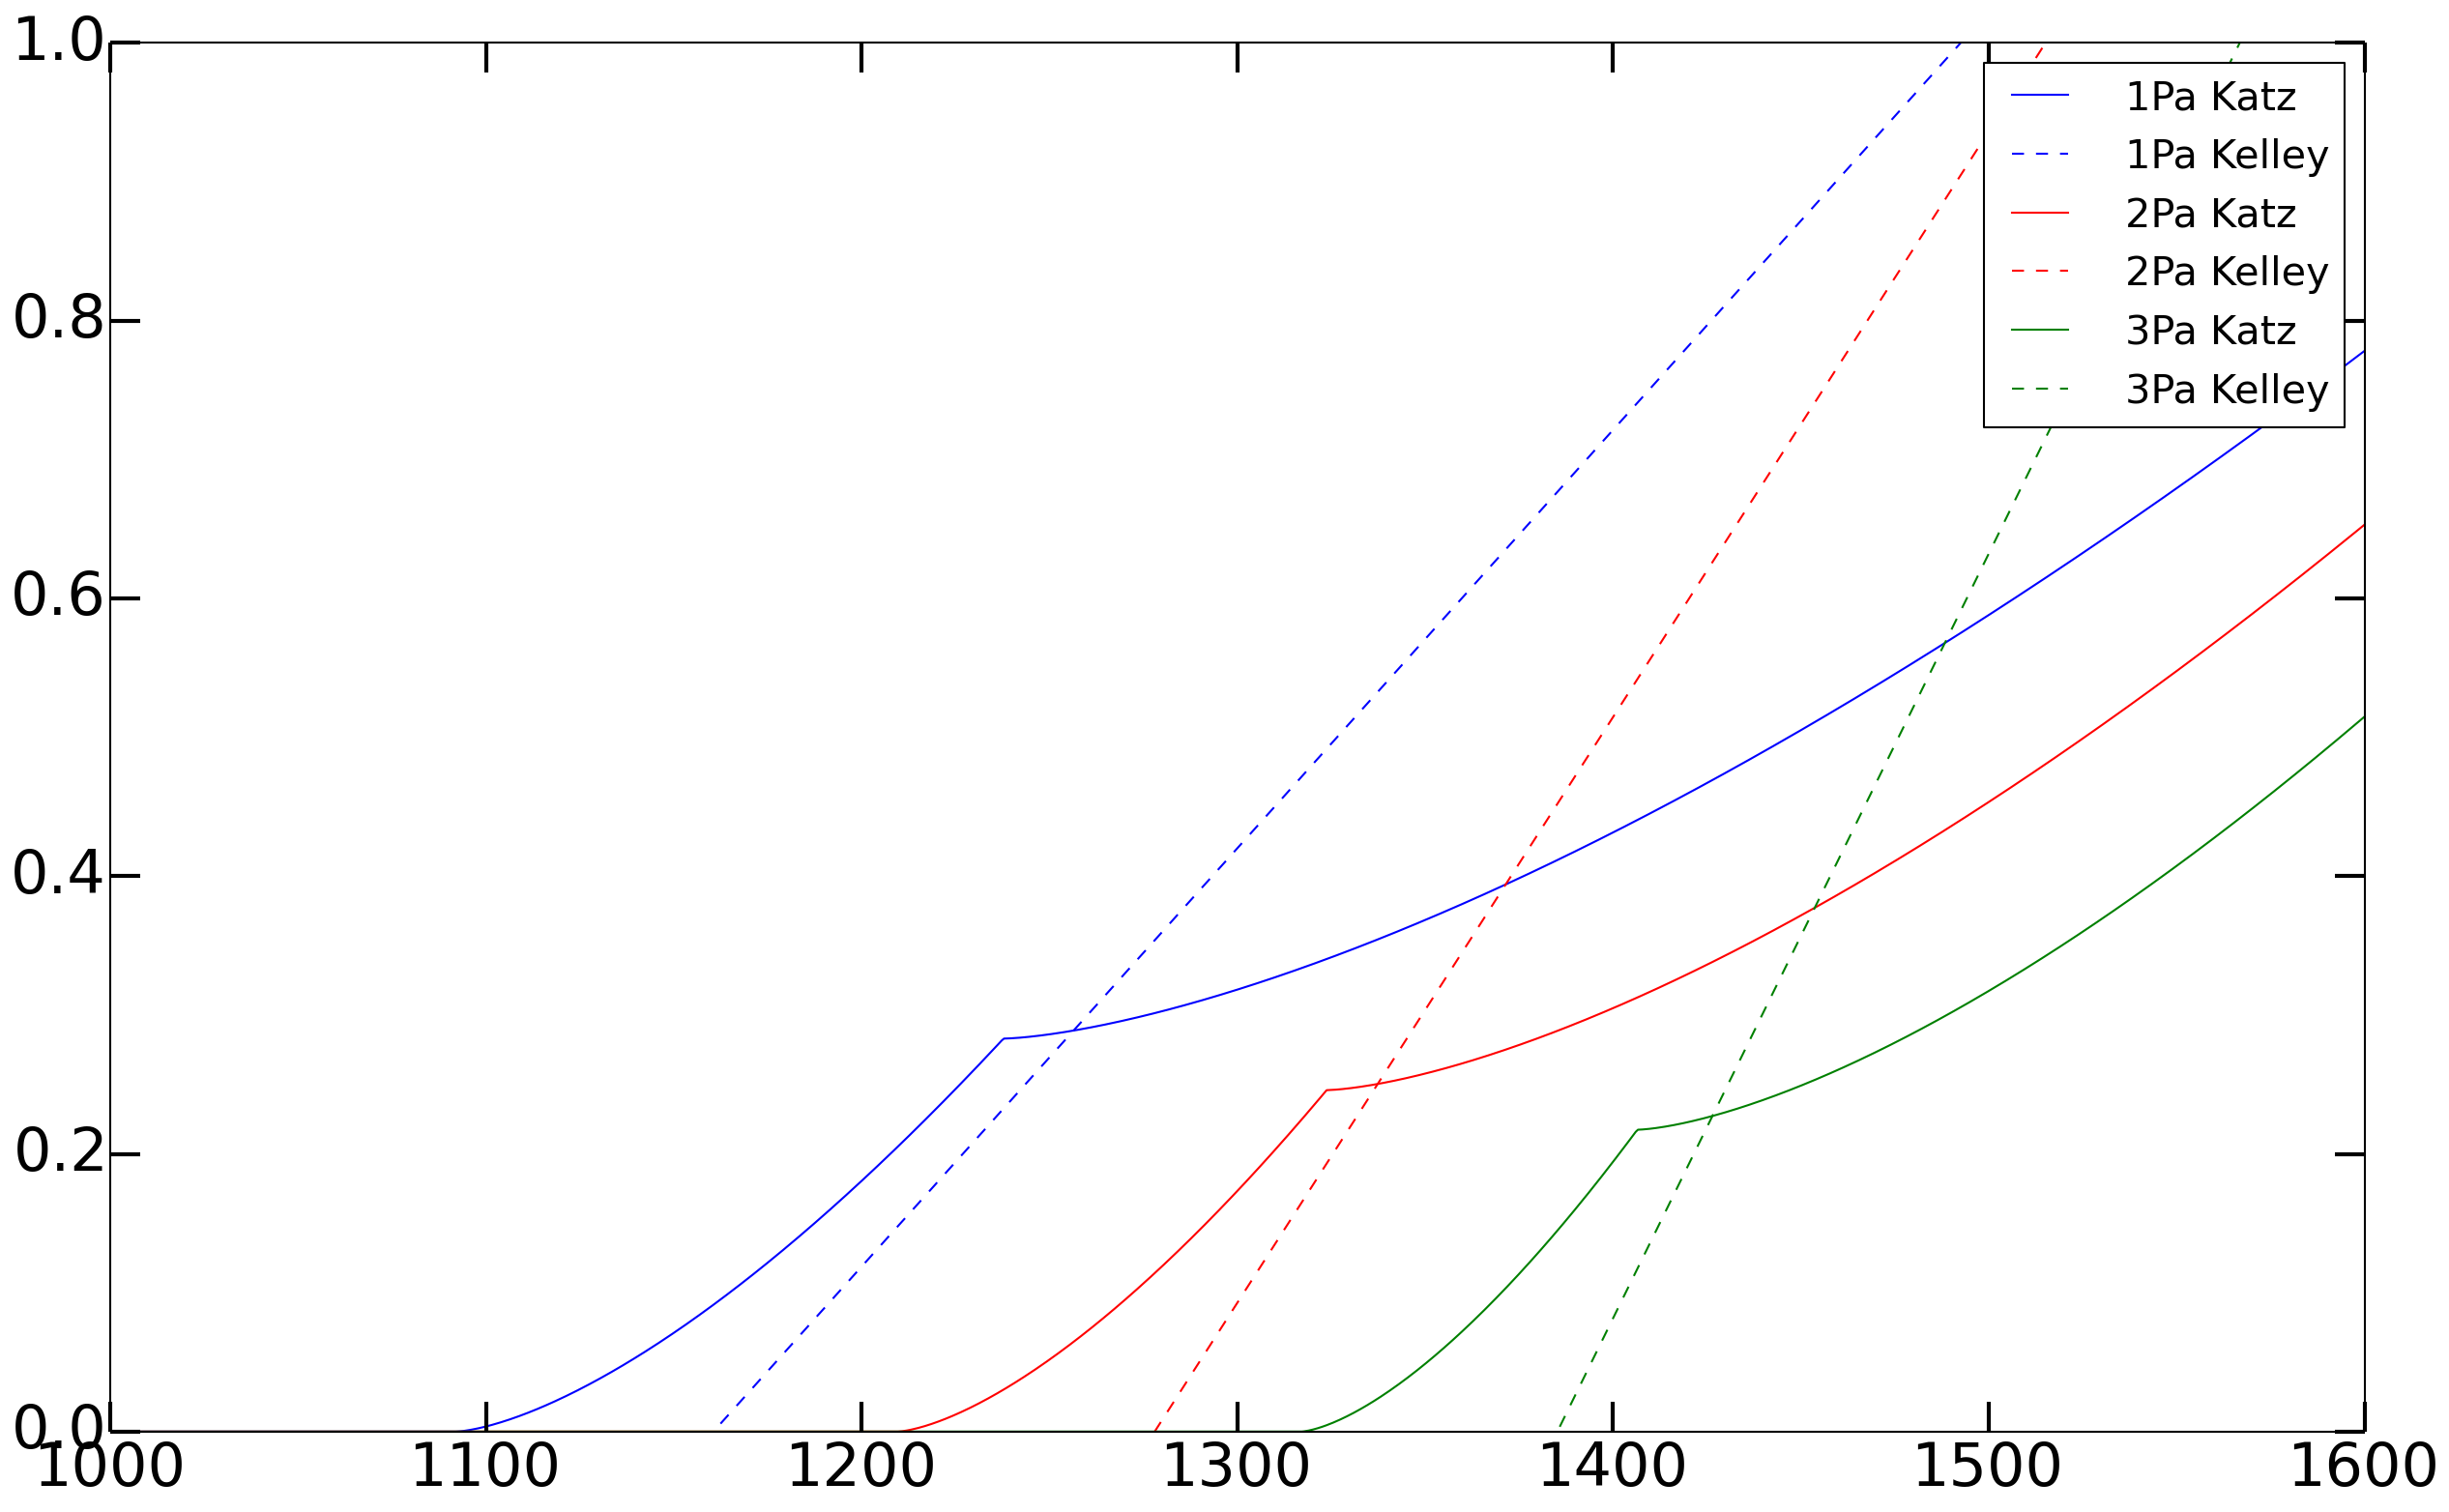
\includegraphics[width=0.9\textwidth]{/data/ap4909/30.10.2013-hot_cold_geochem/sample_testing/southern_marianas/kelley/kelley_katz_comparison/figures/katz_kelley_comparison.png}
\label{ti_resid_v_f}
\captionsetup{singlelinecheck=off}
\caption[]{
\begin{itemize}
\item Assuming 4 wt\% H2O for our samples, 0.25 fo2. 
\end{itemize}
}
\end{figure}

\begin{figure}[H]
%/data/ap4909/30.10.2013-hot_cold_geochem/sample_testing/southern_marianas/kelley/mf_vs_ti.py
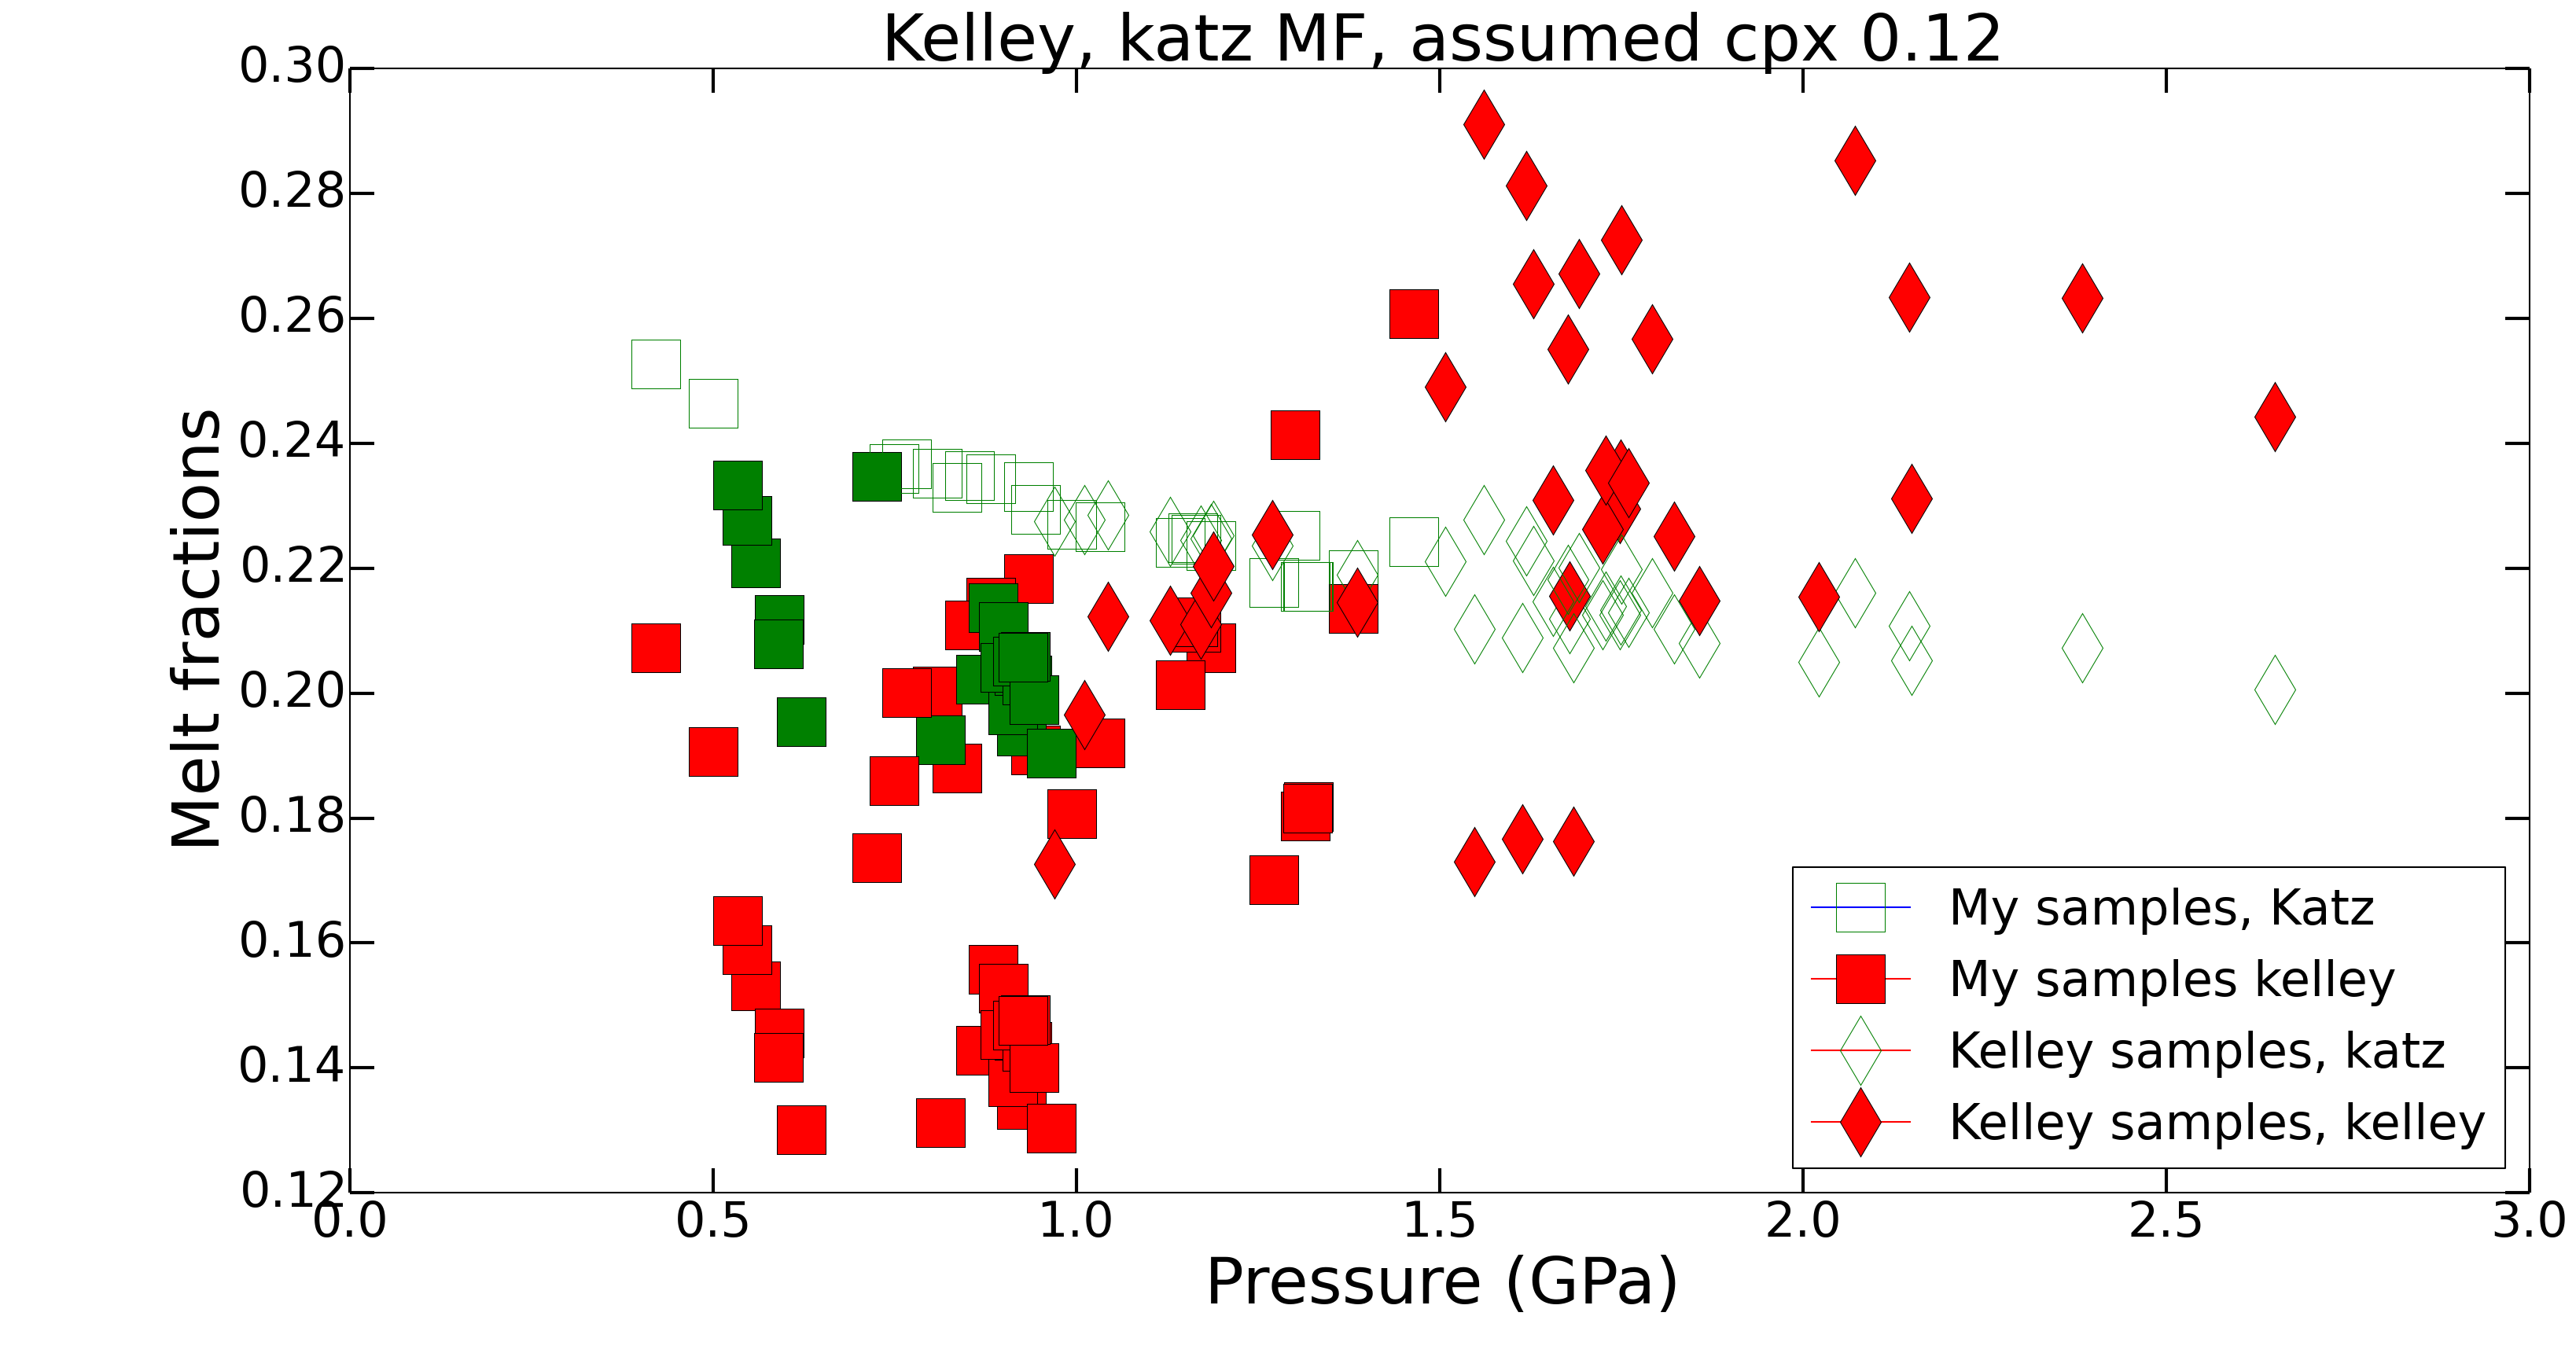
\includegraphics[width=0.9\textwidth]{/data/ap4909/30.10.2013-hot_cold_geochem/sample_testing/southern_marianas/kelley/kelley_katz_comparison/figures/melt_fractions/katz_kelley_mf_vs_P.png}
\label{ti_resid_v_f}
\captionsetup{singlelinecheck=off}
\caption[]{
\begin{itemize}
\item Assuming 4 wt\% H2O for all samples, 0.25 fo2. 

\item hollow symbols - cpx has been exhausted.
\item Below 1GPa Katz MF higher than Kelley MF - due to lower solidus of Katz.
\item Above 1 GPa - Kelley do not consider cpx out - generally higher melt fractions.
\item With increasing pressure, a certain cpx content can be exhausted quicker - this effect is incorporated with Katz, and is why more samples exhaust CPX at increasing pressure.
\item Kelley also have a dT/dF variation with pressure, leading to higher melt productivities at higher pressures.

\end{itemize}
}
\end{figure}
\begin{figure}[H]
%/data/ap4909/30.10.2013-hot_cold_geochem/sample_testing/southern_marianas/kelley/mf_vs_ti.py
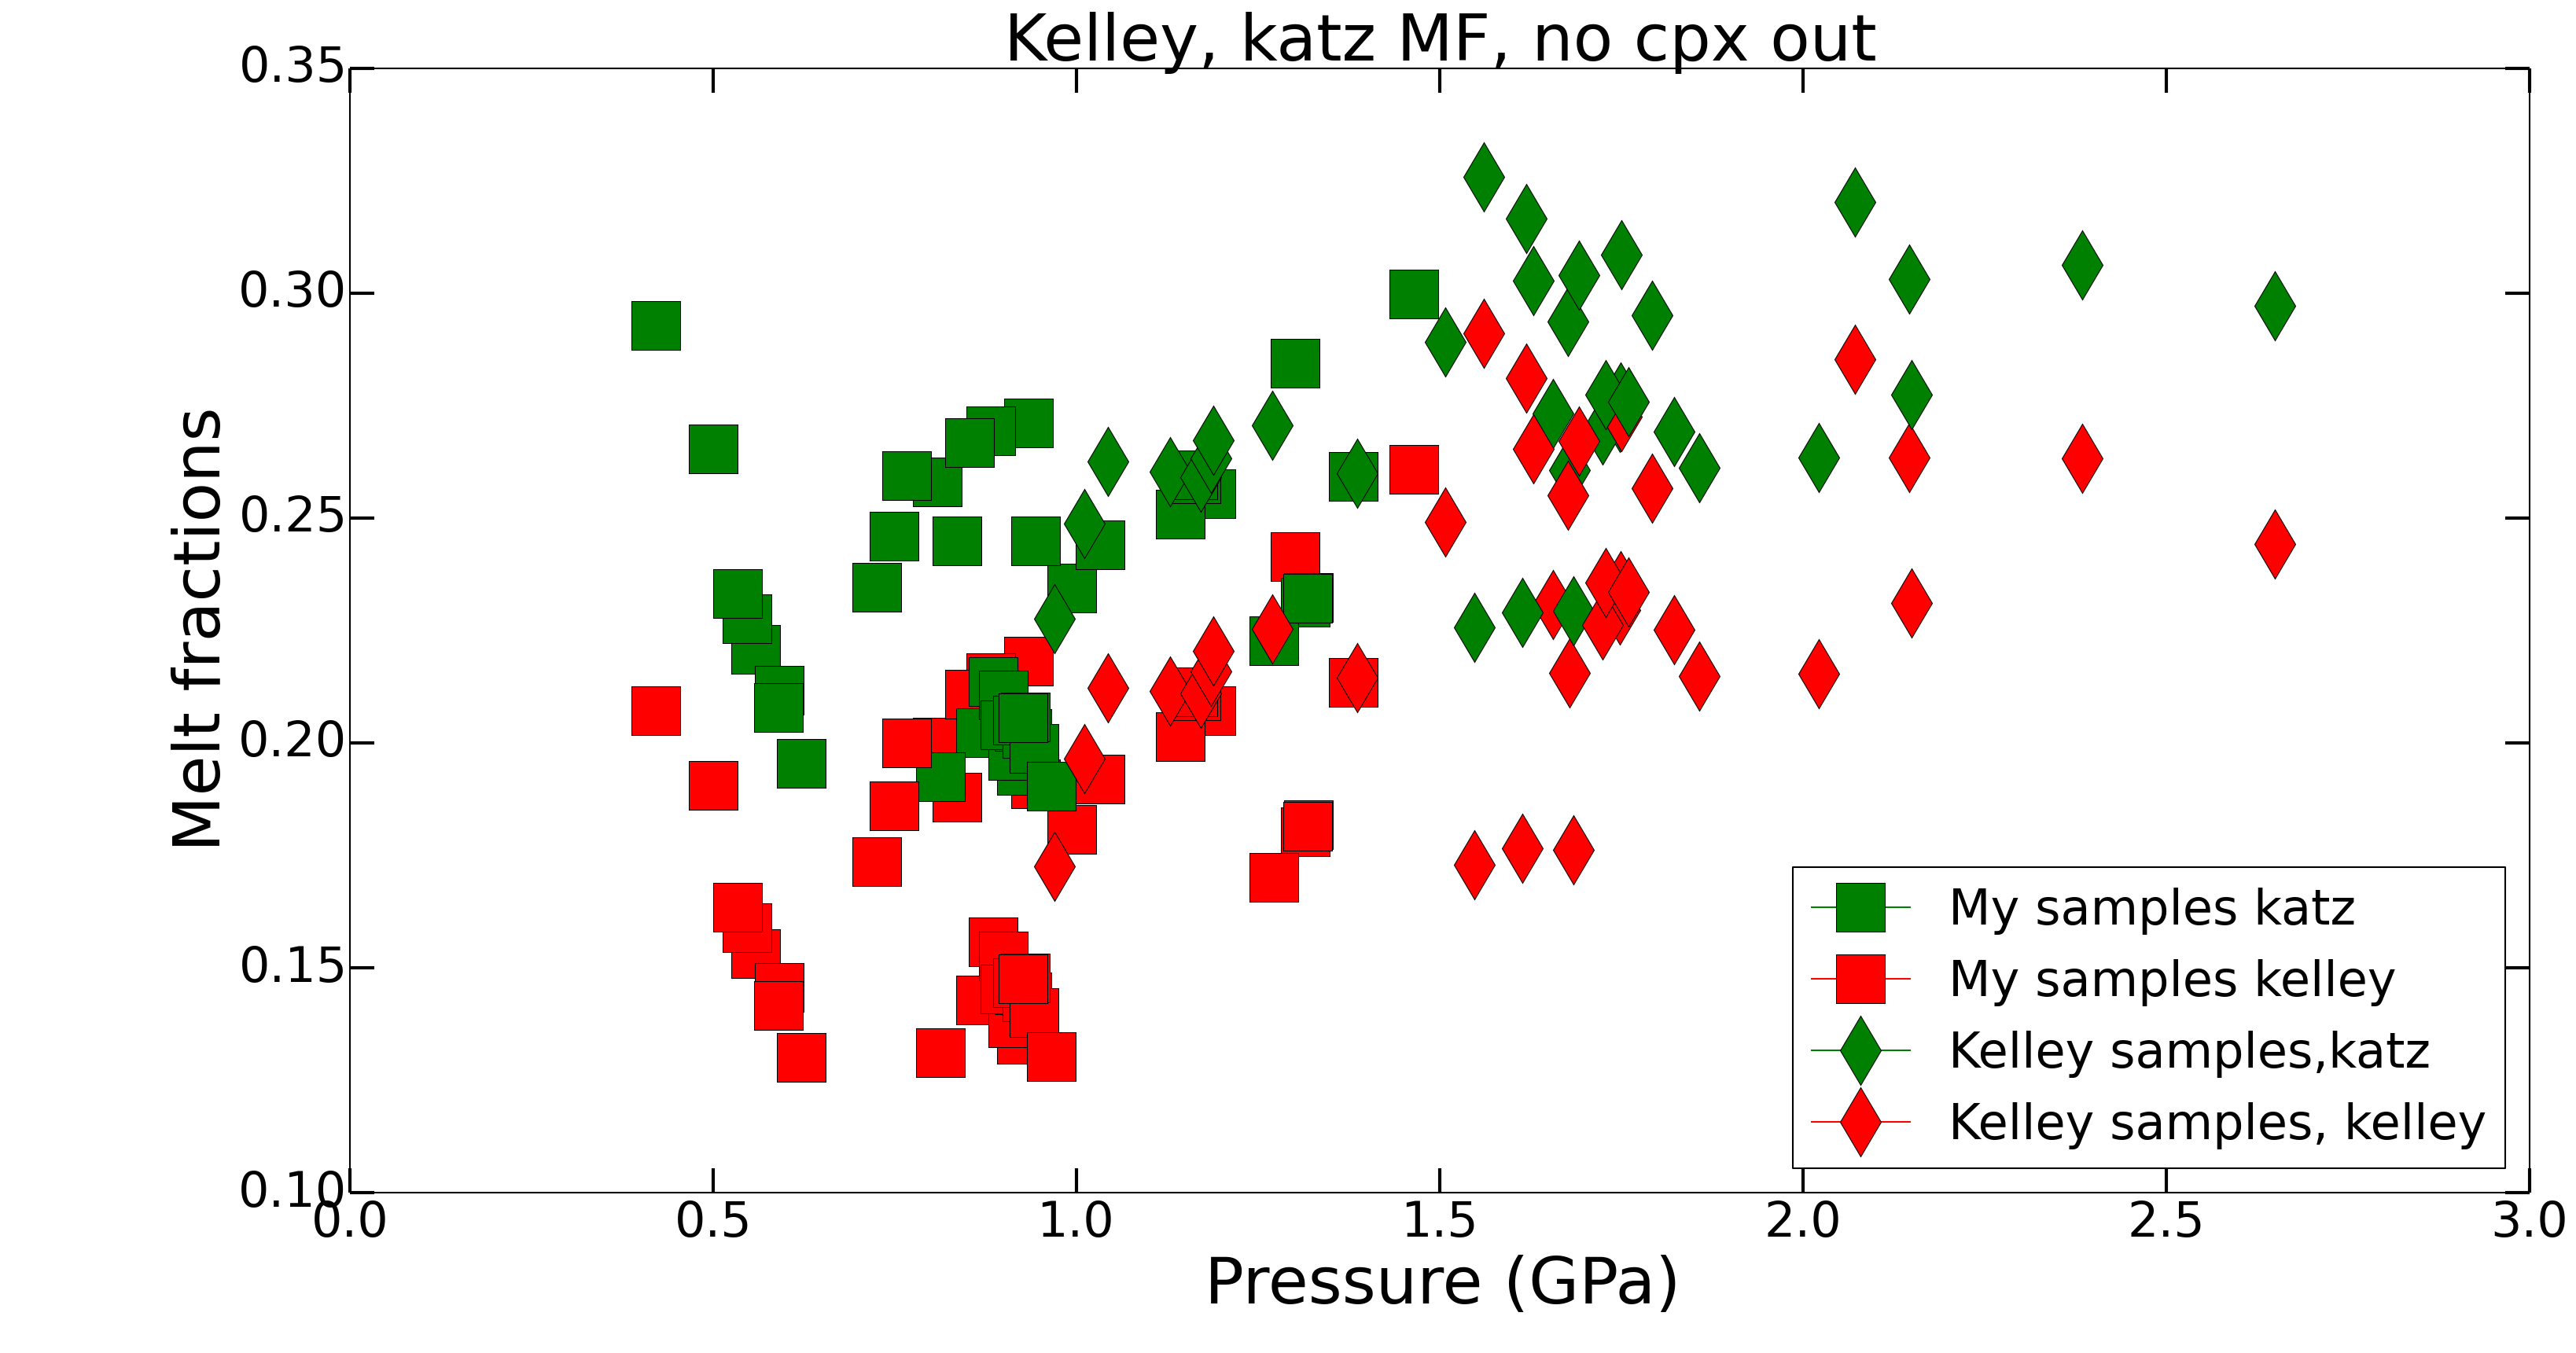
\includegraphics[width=0.9\textwidth]{/data/ap4909/30.10.2013-hot_cold_geochem/sample_testing/southern_marianas/kelley/kelley_katz_comparison/figures/melt_fractions/katz_kelley_mf_vs_P_no_katz_cpx_out.png}
\label{ti_resid_v_f}
\captionsetup{singlelinecheck=off}
\caption[]{
\begin{itemize}
\item Assuming 4 wt\% H2O for all samples, 0.25 fo2. 
\item When cpx exhaustion is excluded from Katz calculation, 
\end{itemize}
}
\end{figure}
\begin{figure}[H]
%/data/ap4909/30.10.2013-hot_cold_geochem/sample_testing/southern_marianas/kelley/mf_vs_ti.py
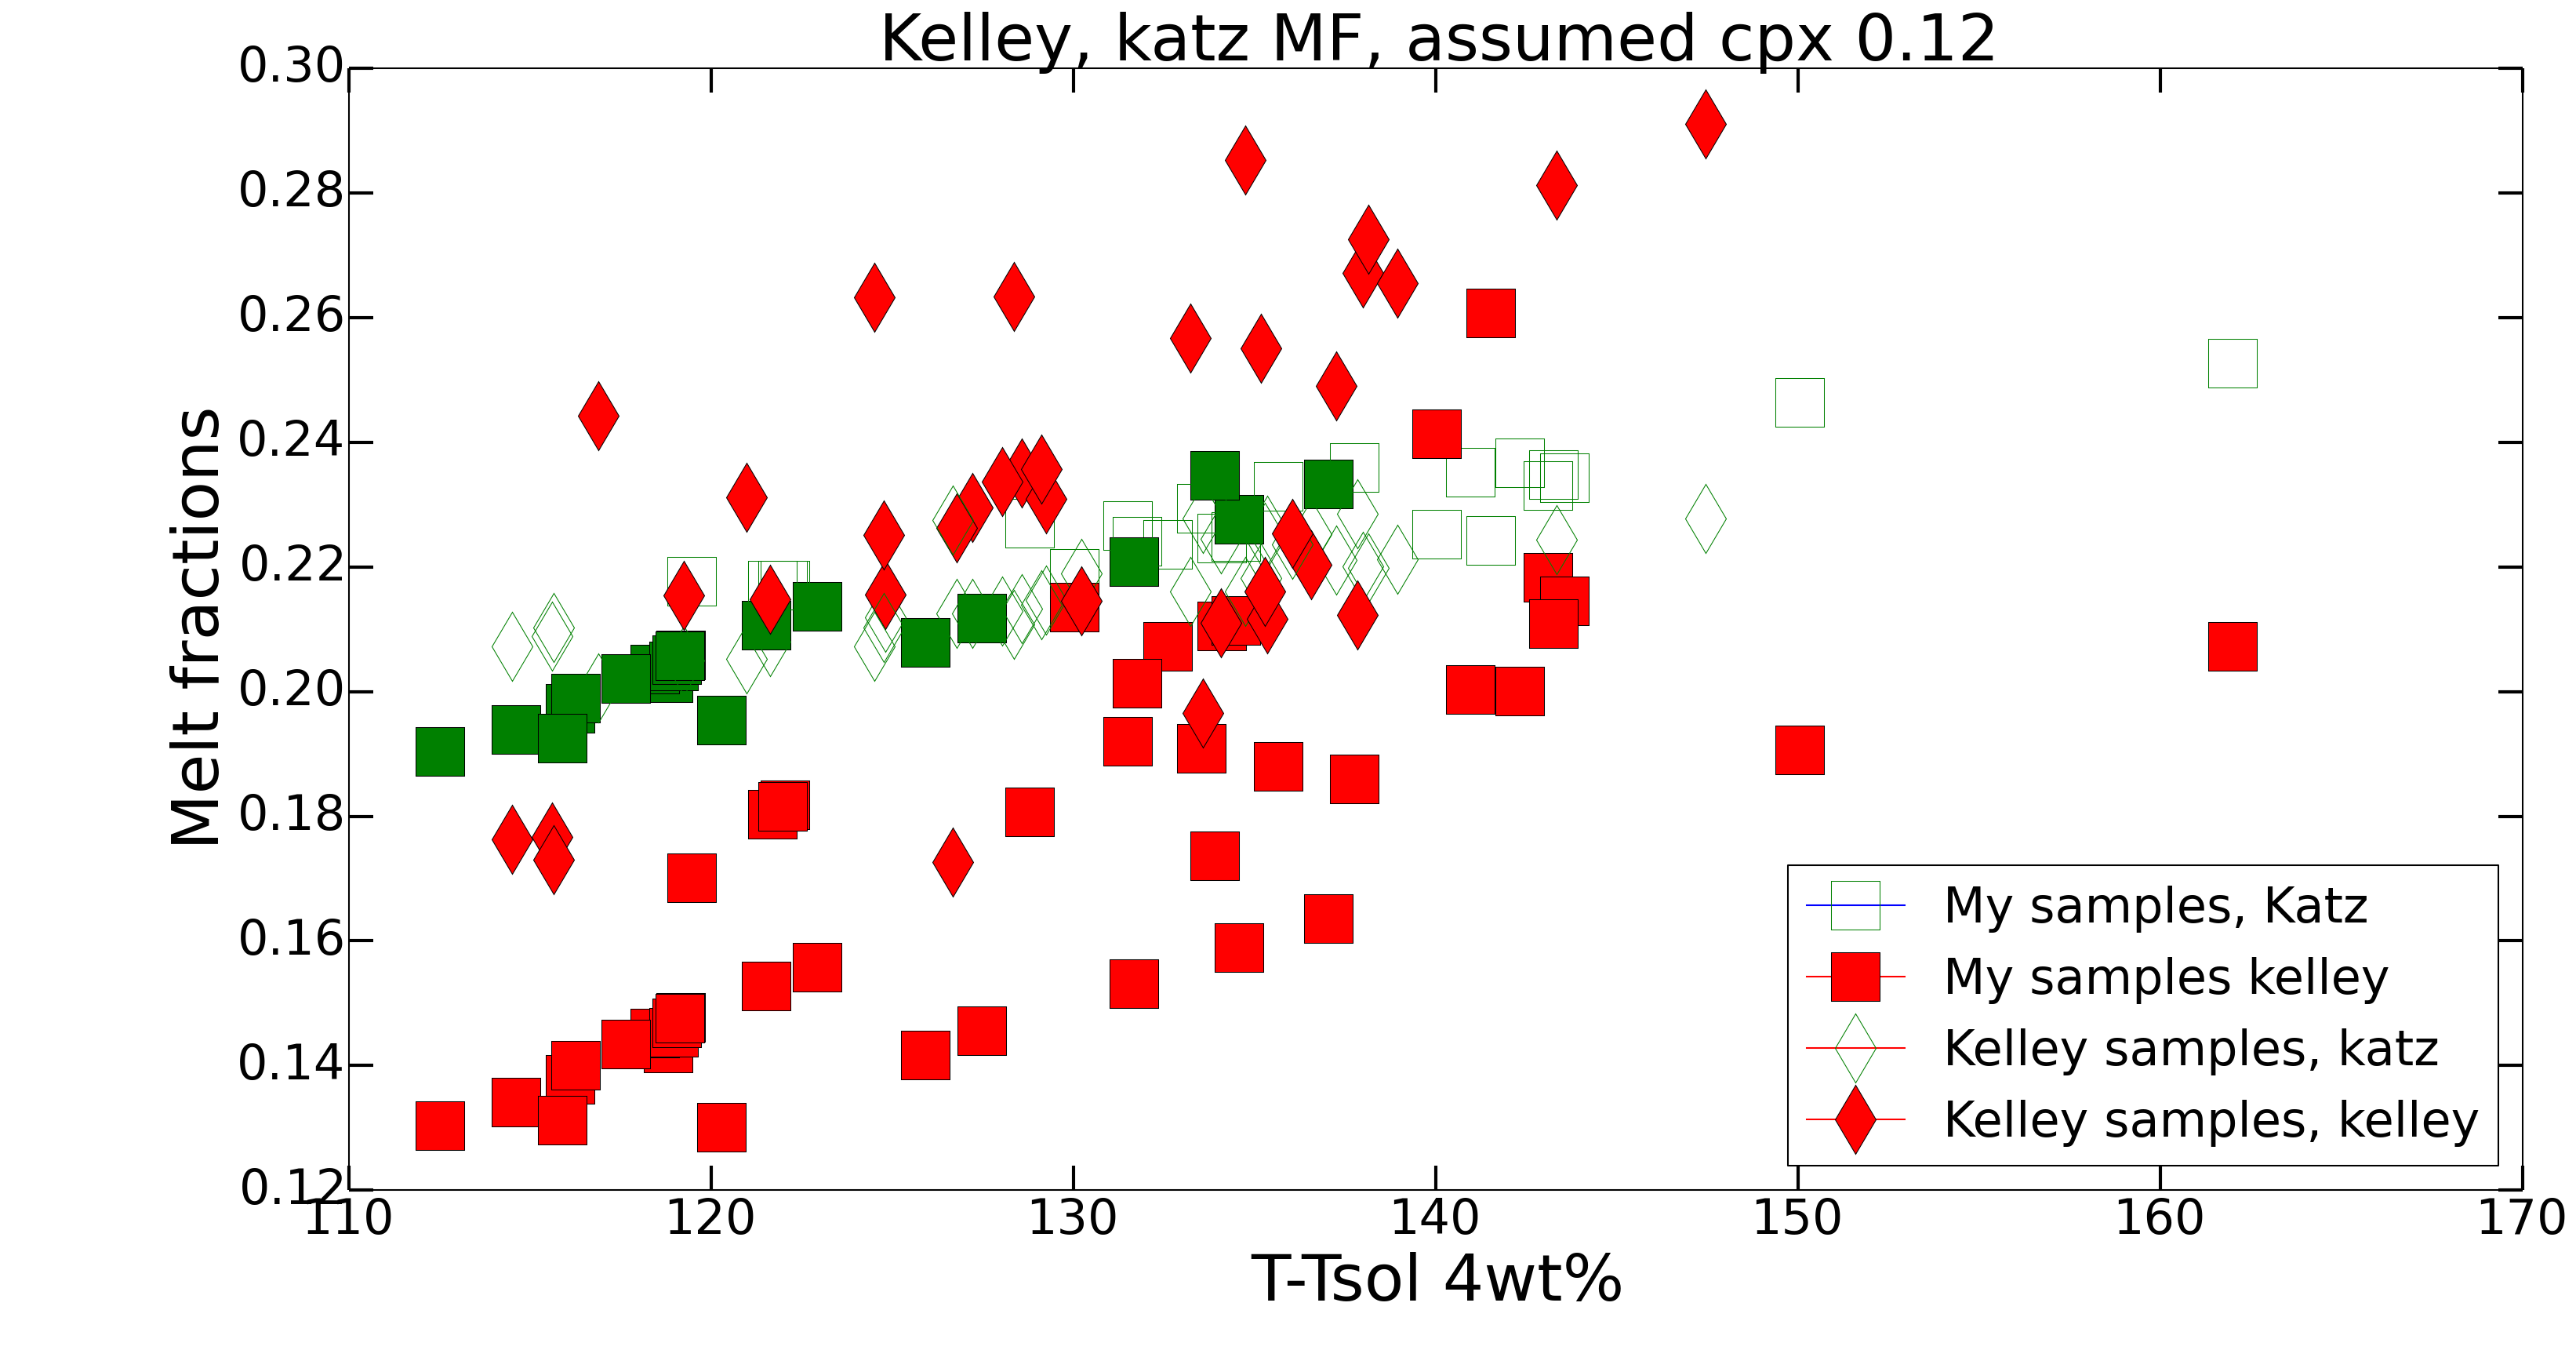
\includegraphics[width=0.9\textwidth]{/data/ap4909/30.10.2013-hot_cold_geochem/sample_testing/southern_marianas/kelley/kelley_katz_comparison/figures/melt_fractions/katz_kelley_mf_vs_t_minus_tsol.png}
\label{ti_resid_v_f}
\captionsetup{singlelinecheck=off}
\caption[]{
\begin{itemize}
\item Assuming 4 wt\% H2O for all samples, 0.25 fo2. 
\item When cpx exhaustion is excluded from Katz calculation, 
\end{itemize}
}
\end{figure}


\begin{figure}[H]
%/data/ap4909/30.10.2013-hot_cold_geochem/sample_testing/southern_marianas/kelley/mf_vs_ti.py
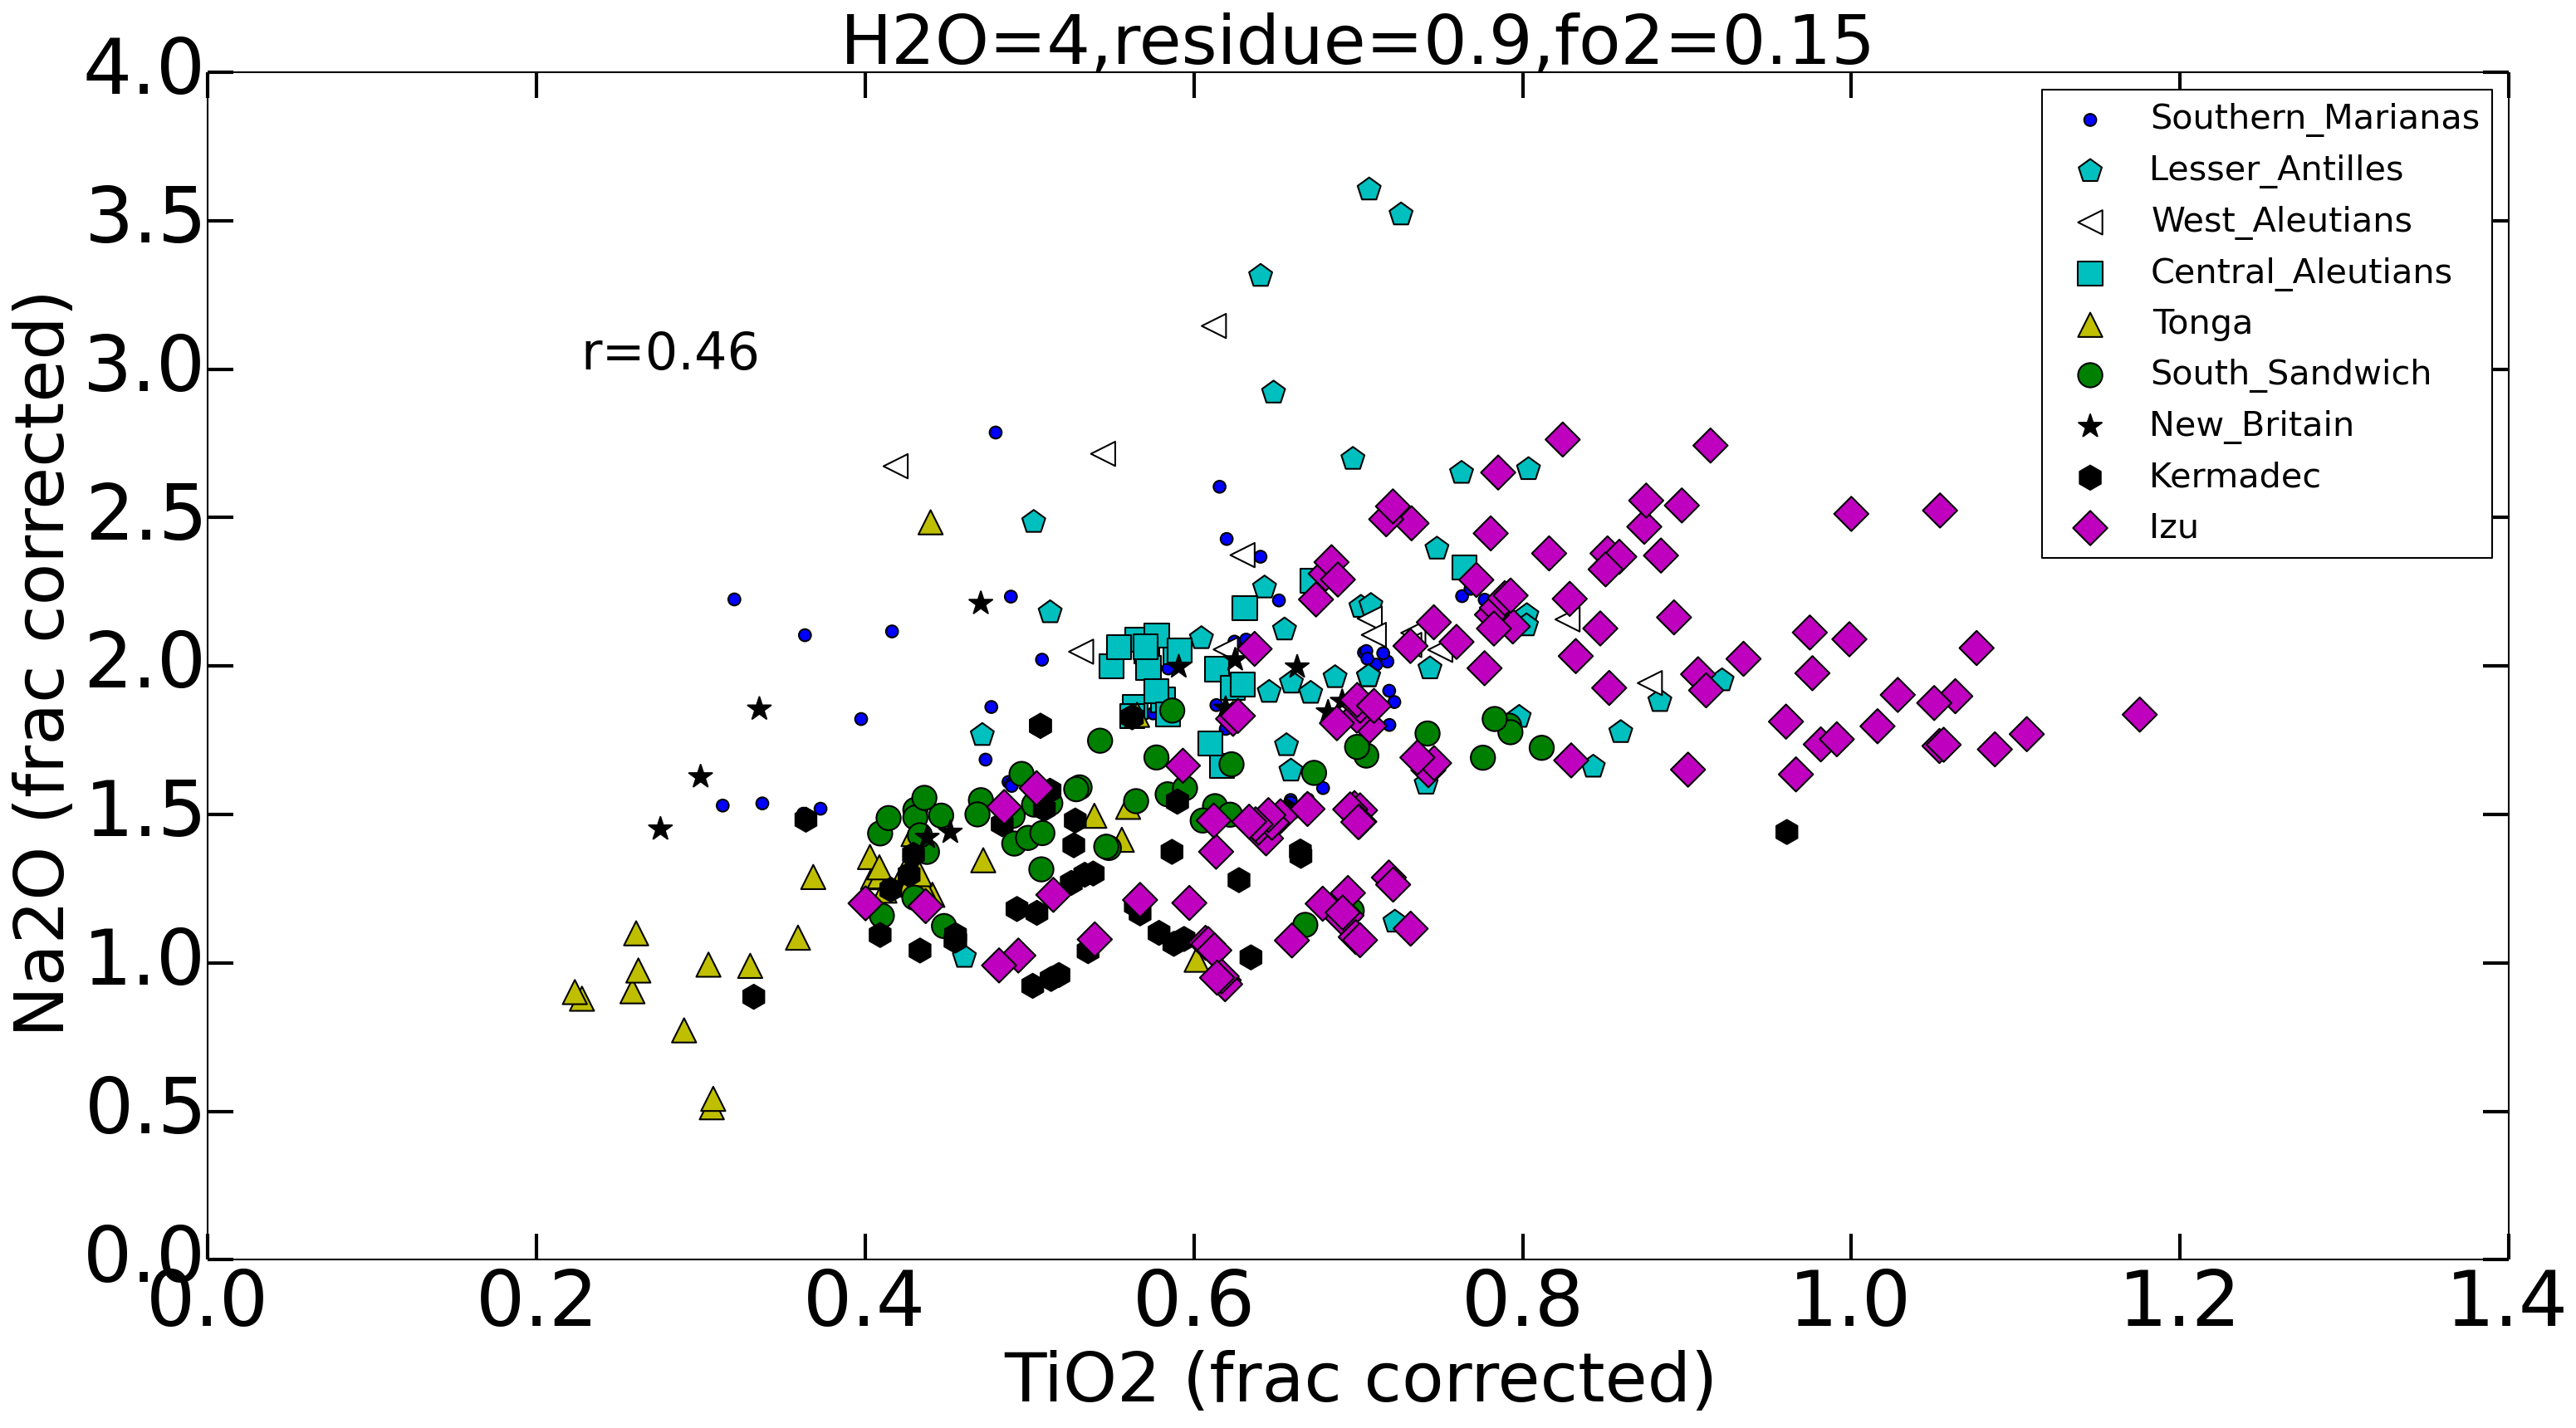
\includegraphics[width=0.9\textwidth]{/data/ap4909/30.10.2013-hot_cold_geochem/sample_testing/southern_marianas/kelley/figures/melt_fractions/na2o_vs_tio2.png}
\label{ti_resid_v_f}
\captionsetup{singlelinecheck=off}
\caption[]{

}
\end{figure}
\begin{figure}[H]
%/data/ap4909/30.10.2013-hot_cold_geochem/sample_testing/southern_marianas/kelley/mf_vs_ti.py
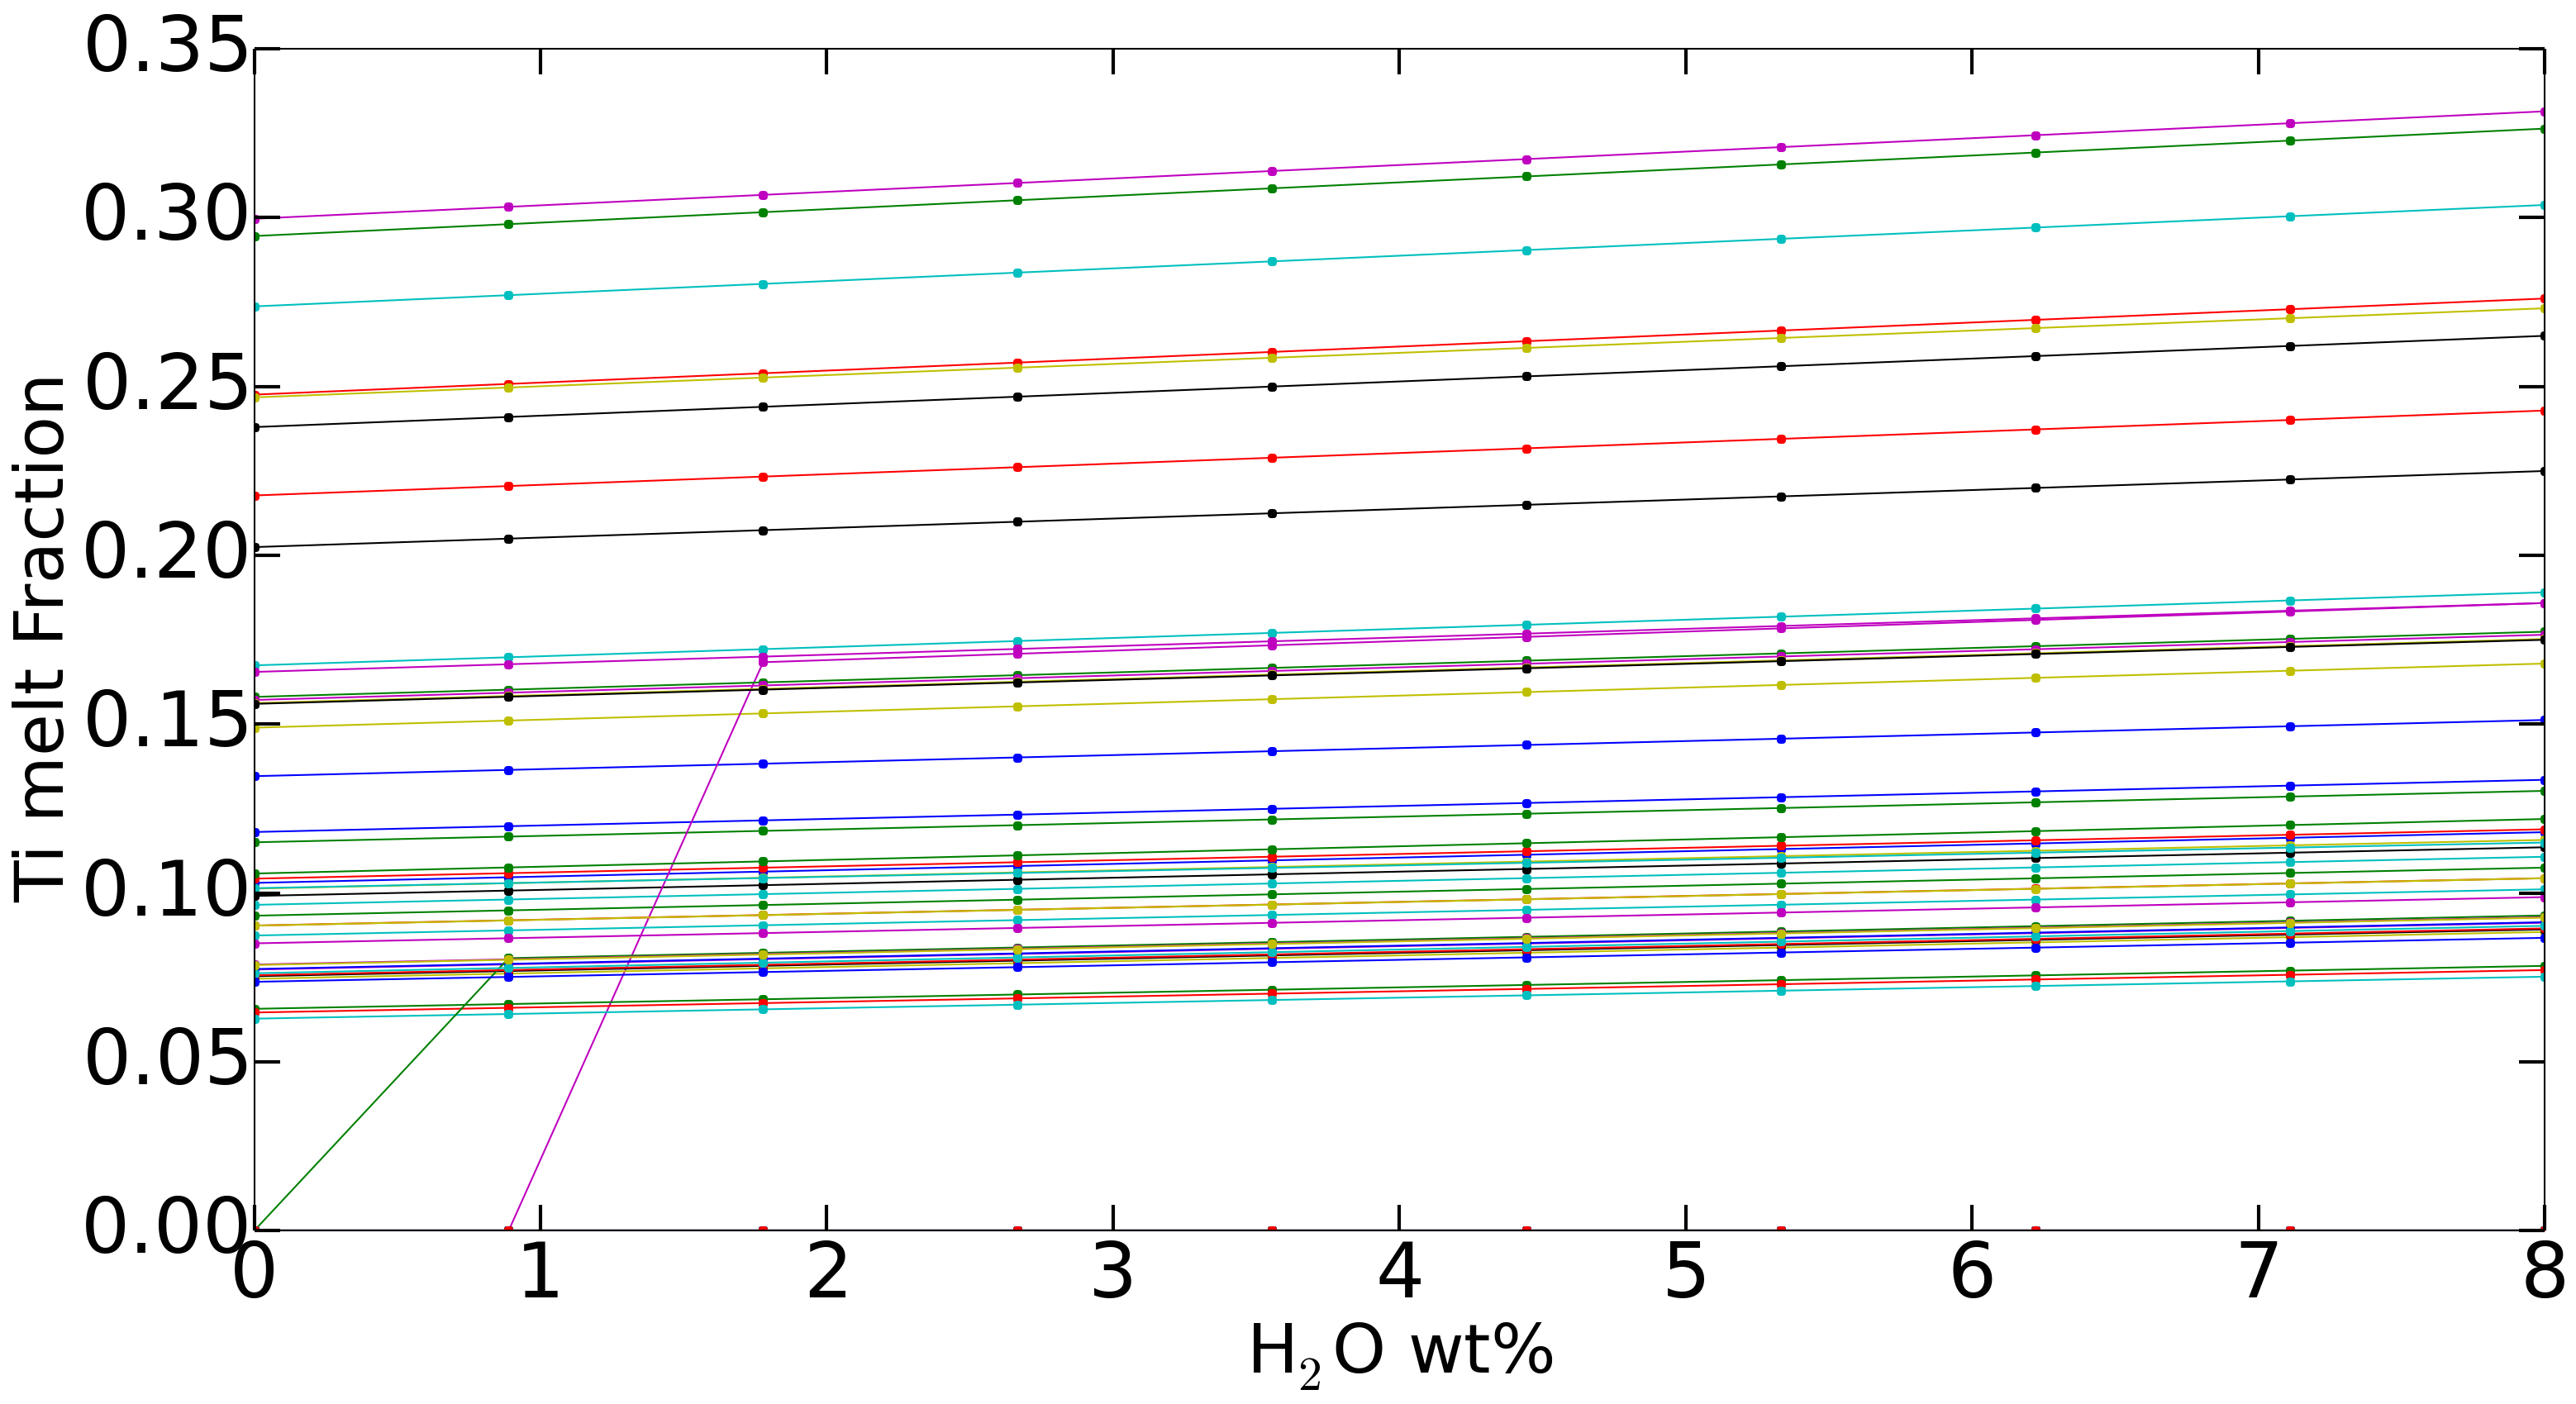
\includegraphics[width=0.9\textwidth]{/data/ap4909/30.10.2013-hot_cold_geochem/sample_testing/southern_marianas/kelley/ti_melt_uncertainties/figures/ti_mf_vs_h2o.png}
\label{ti_resid_v_f}
\captionsetup{singlelinecheck=off}
\caption[]{
\begin{itemize}
\item Changing H$_2$O from 0-8 wt\% results in around 2\% melt increase.
\end{itemize}

}
\end{figure}
\begin{comment}
\begin{figure}[H]
%/data/ap4909/30.10.2013-hot_cold_geochem/sample_testing/southern_marianas/kelley/mf_vs_ti.py
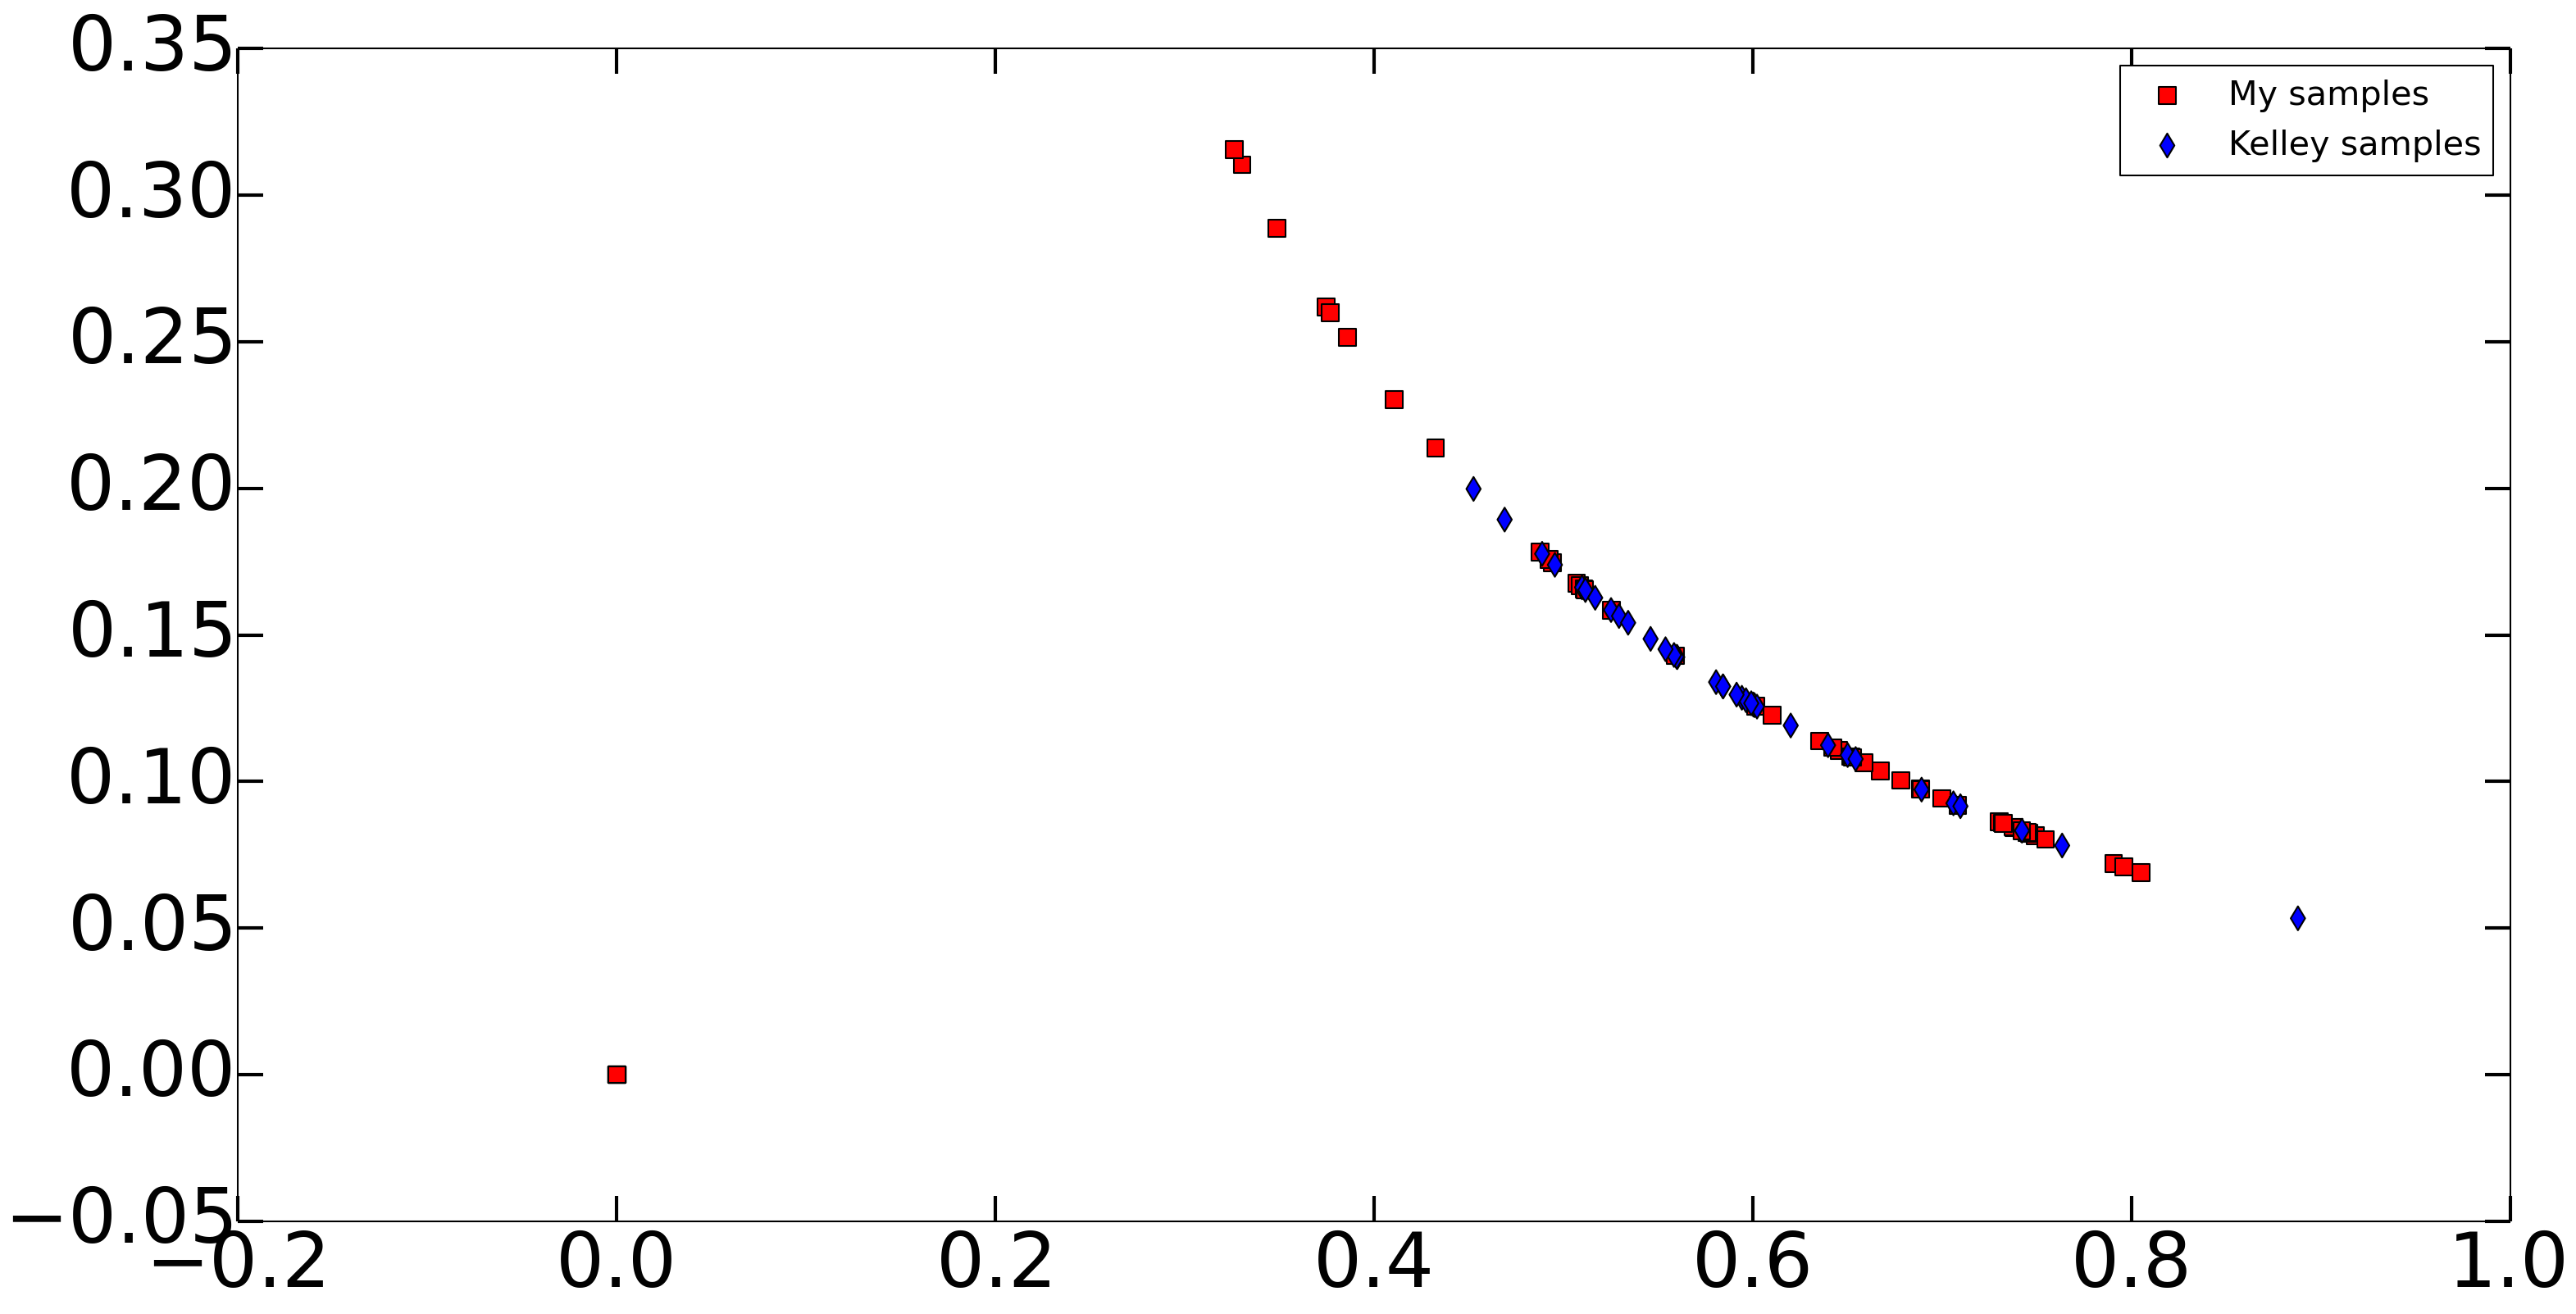
\includegraphics[width=0.9\textwidth]{/data/ap4909/30.10.2013-hot_cold_geochem/sample_testing/southern_marianas/kelley/figures/melt_fractions/mf_vs_ti.png}
\label{ti_resid_v_f}
\captionsetup{singlelinecheck=off}
\caption[]{
\begin{itemize}
\item Assuming 4 wt\% H2O for our samples, 0.123wt\% mantle source Ti, 0.25 fo2.
\end{itemize}
}
\end{figure}
\end{comment}
\bibliography{/home/ap4909/Dropbox/PhD/ongoing_results/2015_ongoing_results/seismic,/home/ap4909/Dropbox/PhD/ongoing_results/2015_ongoing_results/geochemistry,/home/ap4909/Dropbox/PhD/ongoing_results/2015_ongoing_results/geodynamics}
\bibliographystyle{plainnat}
\end{document}